
\documentclass[11pt, oneside]{article} 
\usepackage{amsmath, amsthm, amssymb, wasysym, verbatim, bbm, color, geometry}
\usepackage{amsfonts}
\usepackage{csquotes}
% \usepackage{polski}
\usepackage[english]{babel}
\usepackage[nottoc]{tocbibind}
\usepackage{caption}
\usepackage{subcaption}
\usepackage{float}
\usepackage{graphicx}
\usepackage{circuitikz}
% \ctikzset{current arrow scale=1.5} 
\usepackage{hyperref} % Loads the hyperref package for hyperlinks
\usepackage{enumitem}
\usepackage{tikz}
\usepackage{pgfplots}
\usepackage[T1]{fontenc}
\usepackage{algorithm}
\usepackage{algpseudocode}
\usepackage{amsfonts}
\usepackage{mathbbol}


\pgfplotsset{compat=1.18} % Set the compatibility level for pg
\usetikzlibrary{shapes.geometric, arrows, positioning, fit, backgrounds}

\hypersetup{
    colorlinks=true,
    linkcolor=blue,
    citecolor=cyan,
    urlcolor=blue!60,
    breaklinks=true,
}





\newcommand{\workSource}[2]{Text available at: \href{#1}{#2}}



\DeclareMathSizes{12}{12}{10}{8}
\makeatletter
\renewcommand\normalsize{%
\@setfontsize\normalsize{12pt}{13.5pt}% Will look incredibly crabbed if line height is too small
\abovedisplayskip 10\p@ \@plus2\p@ \@minus5\p@%
\abovedisplayshortskip \z@ \@plus2\p@%
\belowdisplayshortskip 5\p@ \@plus2\p@ \@minus3\p@%
\belowdisplayskip \abovedisplayskip%
\let\@listi\@listI%
}
\normalsize  
\makeatother

\newcommand{\der}{{\rm d}}
\newcommand{\R}{\mathcal{R}}
\newcommand{\C}{\mathcal{C}}
\newcommand{\M}{\mathcal{M}}
\newcommand{\G}{\mathcal{G}}
\newcommand{\Ron}{R_{\rm ON}}
\newcommand{\Roff}{R_{\rm OFF}}
\newcommand{\von}{V_{\rm ON}}
\newcommand{\voff}{V_{\rm OFF}}
\newcommand{\q}{q}
\newcommand{\ua}{v}
\newcommand{\ia}{i}
\newcommand{\phia}{\varphi}
\newcommand{\xw}{x}
\newcommand{\dert}[1]{\frac{{\rm d} {#1}}{{\rm d} t} }
\newcommand{\inv}[1]{\frac{1}{#1} }
\newcommand{\equal}{=}


\usepackage[style=numeric, 
            backend=biber,
           ]{biblatex}
           
\addbibresource{bibliography.bib} % Replace with your .bib file name

\geometry{tmargin=.75in, bmargin=.75in, lmargin=.75in, rmargin = .75in}  

% \usepackage{fontspec}
% \setmainfont[]{Palatino}

\newcommand{\Cdot}{\boldsymbol{\cdot}}

\newtheorem{thm}{Theorem}
\newtheorem{defn}{Definition}
\newtheorem{conv}{Convention}
\newtheorem{rem}{Remark}
\newtheorem{lem}{Lemma}
\newtheorem{cor}{Corollary}


\title{Modeling SDC Memristors Using Artificial Neural Networks}
\author{Karol Bednarz}
% \date{Rok akademicki 2024--2025}
\date{\today}

\begin{document}

\maketitle
\tableofcontents

\vspace{.25in}

\newcommand{\Todo}[1]{\textcolor{red}{\textbf{TODO:} #1}}

\section{Introduction}


Numerous memristor models have been proposed in the scientific literature following the discovery of memristive behavior at the nanoscale. The original model, introduced in~\cite{Strukov2008}, conceptualizes the memristor as a series connection of two variable resistances corresponding to the conductive and insulating regions of the thin film. To more accurately model Self-Directed Channel (SDC) memristors, M.~Nugent and T.~Molter proposed the generalized \textit{Mean Metastable Switch} (MMS) model, which is a semi-empirical formulation. In this approach, the time derivative of the internal state variable is defined as a function of both the transition probabilities between metastable states and the current value of the state variable~\cite{Molter2016}. In~\cite{Lee2024}, the authors attempted to model memristive behavior using the \textit{Physics-Informed Neural Networks} (PINNs) framework. Although the reported results indicate the potential of this method, the study is not grounded in experimental measurements of physical memristor devices. Instead, the analysis is limited to comparisons with the outcomes of existing simulation models. Moreover, the training data employed during the neural network learning process were generated based on previously developed theoretical models, thereby limiting the ability to assess the method's accuracy in the context of real-world physical systems.



In~\cite{Ricky2018}, the authors introduce the concept of deep neural models in which the dynamics of the hidden state are governed by an \textit{ordinary differential equation} (ODE). The training process is performed in an end-to-end manner, meaning that all parameters are optimized simultaneously within a single training routine. A key innovation of the proposed approach is a novel backpropagation technique, which relies on solving the corresponding adjoint ODE backward in time using \textit{adjoint sensitivity methods}. This formulation enables efficient gradient computation and facilitates the application of neural ODEs in various architectures, including continuous-depth residual networks and generative flow-based models.

In~\cite{Ricky2021}, the authors extend the classical Neural ODE framework to enable the modeling of discontinuous events in continuous time—without requiring prior knowledge of the number or timing of such events. The proposed differentiable event functions allow for efficient simulation of hybrid systems, such as systems with collisions, state-switching mechanisms, or point processes. This development opens up new possibilities for modeling and training systems with discrete control inputs and non-smooth dynamics.

\Todo{Add more information about the referenced work, including applications and results.}

The present study aims to investigate the feasibility of modeling Self-Directed Channel (SDC) memristors using artificial neural networks, and to compare the effectiveness of this approach with that of existing theoretical models. Specifically, we focus on the application of Neural Ordinary Differential Equation (Neural ODE) models to simulate the behavior of SDC memristors, utilizing experimental data obtained from real physical systems.

Our objective is to assess whether neural network-based models can accurately reproduce the dynamic characteristics of SDC memristors, and to determine whether they offer any advantages over traditional theoretical approaches—particularly in terms of modeling flexibility, accuracy, and applicability to real-world, measurement-driven scenarios.

\section{Materials and Methods}


\subsection{Memristors and Measurement Procedure}

This study utilizes experimental data obtained from physical Self-Directed Channel (SDC) memristors doped with tungsten. The structure and properties of these devices have been described in detail in the literature, e.g., in~\cite{Garda2024, Campbell2017}.

The experimental setup, illustrated in Fig.~\ref{fig:memristor_setup}, consisted of an SDC memristor connected in series with a resistor. The sinusoidal input voltage was supplied by an arbitrary waveform generator, while the voltage signals were measured using a data acquisition (DAQ) system.

Measurements were carried out for various combinations of supply voltage amplitudes and frequencies. Specifically, the amplitude of the applied voltage was varied as $V_s \in \{0.5,\ 1.0,\ 1.5\}~\mathrm{[V]}$, and the frequency was selected from the set $f \in \{1,\ 5,\ 10,\ 20,\ 50,\ 100\}~\mathrm{[Hz]}$.


\begin{figure}[H]
    \centering
    \resizebox{0.5\linewidth}{!}{%
        
\begin{circuitikz}[american, cute inductors, transform shape]
  \draw (0, 0)
  to [vsourcesin, fill=blue, l=\(v_s \equal V_s\sin (2 \pi f_s \cdot t)\)] (1,0)
  to  [memristor, fill=yellow, l=\(M\), v=\(v_{m}\), invert] (4,0)
  to [short, i=\(i_{m}\)] (4.5,0)
  to [R, l=\(R_s\), v=\(v_{r}\)] (6.5,0);
  \draw (0,0) -- (-0.5,0) node[rground]{};
  \draw (6.5,0) -- (7,0) node[rground]{};
  \draw (0,-2.5);
\end{circuitikz}}
    \vspace{-0.5in}
    \caption{Schematic diagram of the measurement setup used for the SDC memristor. The device is connected in series with a resistor, and the input voltage is applied via an arbitrary waveform generator. Voltage measurements are acquired using a data acquisition (DAQ) system.}
    \label{fig:memristor_setup}
\end{figure}

\subsection{Modeling with Neural Networks}
The analyzed model is based on a general description of a memristive device, formulated using the equations~\eqref{eq:memristor_model1} and~\eqref{eq:memristor_model}.


\newcommand{\xvec}{\mathbf{x}}
\begin{align}
    \label{eq:memristor_model1}
    \ua(t)                    & = \M \big(\xvec(t),\ua(t)\big) \, \ia(t), \\
    \label{eq:memristor_model}
    \frac{\der \xvec}{\der t} & = f\big(\xvec(t),\ua(t)\big)
\end{align}
where $\xvec$ denotes the vector of internal state variables, whose temporal evolution is governed by the dynamic function $f$, and $\M$ represents the memristance of the device. A fundamental challenge in memristor modeling lies in accurately identifying the functional forms of $\M(\xvec,\ua)$ and $f(\xvec,\ua)$.

In this study, two modeling approaches are considered.
The first approach is deterministic. In self-directed channel (SDC) memristors, the resistance evolves due to the migration of $\mathrm{Ag^+}$ ions and the dynamic formation of conductive filaments. As a consequence, the device conductance undergoes a continuous transition between distinct resistance states. This conductance can be expressed as a weighted combination of the extreme resistance values, modulated by the internal state variable. Specifically, the memristor conductance $G_m(x) = \M(x)^{-1}$ is given by:

\begin{equation}
    G_{m}(x) = \frac{x}{R_{\rm ON}} + \frac{1 - x}{R_{\rm OFF}},
    \label{eq:conductance}
\end{equation}
where $\Ron$ and $\Roff$ denote the resistances in the low-conductance and high-conductance states, respectively.

The second approach employs a data-driven methodology. Here, the memristor conductance is modeled using a neural network, which is trained to capture the nonlinear and complex dependencies between the internal state variables and the applied voltage.

For all of theese aproches also the function $f(\xvec(t), \ua(t))$ was implemented using an artificial neural network, whose conceptual architecture is illustrated in Fig.~\ref{fig:nn_structure}. The neural network consists of interconnected nodes (neurons) that process information through weighted connections. Each neuron in the network computes its output according to:

\begin{equation}
    y = \sigma\left(\sum_{i=1}^{n} w_i x_i + b\right)
\end{equation}

where $w_i$ are the weights that determine the strength and importance of each input connection $x_i$, $b$ is the bias term that provides an adjustable threshold for neuron activation, and $\sigma$ is the activation function (e.g., sigmoid, ReLU, or tanh) that introduces non-linearity into the model.

The weights represent the learnable parameters that encode the relationship between inputs and outputs, while biases allow neurons to shift their activation threshold, enabling the network to better fit the training data even when all inputs are zero. During the optimization process, the network parameters (weights and biases) are tuned jointly with the values of $R_{\rm ON}$ and $R_{\rm OFF}$.

The learning process involves iteratively adjusting the network parameters to minimize a loss function that quantifies the difference between predicted and target outputs. This is  achieved through backpropagation algorithm combined with gradient descent optimization, where gradients of the loss function with respect to each parameter are computed and used to update the weights and biases in the direction that reduces the overall error.

\begin{figure}[H]
    \centering
    \begin{subfigure}[b]{0.49\textwidth}
        \includegraphics[width=\textwidth]{figs/Rysowanie_schematów (1).pdf}
        \label{fig:nn_structure}
        \caption{}
    \end{subfigure}
    \begin{subfigure}[b]{0.49\textwidth}
        \resizebox{\linewidth}{!}{%
            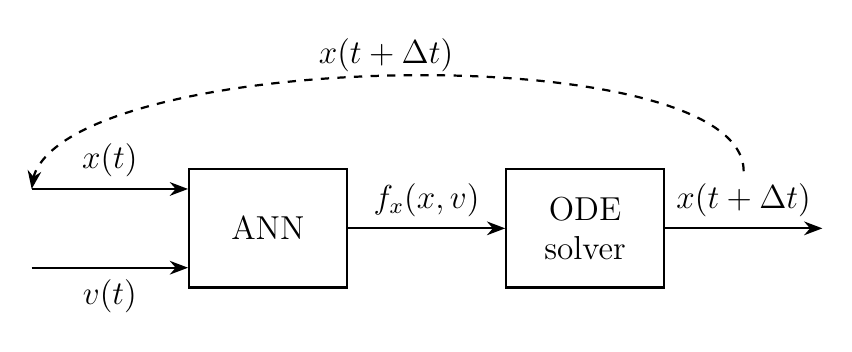
\begin{tikzpicture}[
  node distance=2cm,
  arrow/.style={-{Stealth}, thick,black},
  box/.style={rectangle, draw=black, thick, minimum width=2cm, minimum height=1.5cm, align=center},
  curved/.style={rectangle, draw=black, thick, rounded corners=1cm, minimum width=2cm, minimum height=1.5cm, align=center},
  label/.style={black, font=\large},
  dashed_arrow/.style={-{Stealth}, thick,black, dashed}
  ]
  % Define nodes
  \node[box, label] (ann) {ANN};
  \node[box, label, right=of ann] (ode) {ODE\\solver};
  % Input arrows and labels
  \draw[arrow] (-3, 0.5) -- (ann.west |- 0, 0.5) node[midway, above, label] {$x(t)$};
  \draw[arrow] (-3, -0.5) -- (ann.west |- 0, -0.5) node[midway, below, label] {$v(t)$};
  % Connection between ANN and ODE solver
  \draw[arrow] (ann.east) -- (ode.west) node[midway, above, label] {${f_x}(x,v)$};
  % Output arrow
  \draw[arrow] (ode.east) -- ++(2, 0) node[midway, above, label] (end) {$x(t + \Delta t)$};

  % Dashed feedback line
  \draw[dashed_arrow] (end) to[out=90, in=90, looseness=0.5] (-3, 0.5);
  \node[label] at (1.5, 2.2) {$§          x(t + \Delta t)$};



  % % Dashed boundary
  % \node[draw=black, dashed, thick, rounded corners=0.5cm, fit=(ann) (ode), inner sep=0.8cm] {};
\end{tikzpicture}
        }
        \caption{}
        \label{fig:nn_process}
    \end{subfigure}
    \hfill
    \caption{(a) Conceptual diagram illustrating the use of a neural network to simulate the dynamics of the memristor. (b) Schematic representation of the Neural ODE framework, where an artificial neural network (ANN) computes the derivative function $f_x(x,v)$, which is then integrated by an ODE solver to predict the state at the next time step $x(t + \Delta t)$. The dashed feedback loop indicates the recurrent nature of the process, where the output state is fed back as input for subsequent predictions.}
\end{figure}



The neural network model development and training pipeline was implemented using the \texttt{PyTorch} deep learning framework within the \texttt{Python} programming environment, leveraging its automatic differentiation capabilities and GPU acceleration for efficient computational processing.

% \subsubsection{Differential Equation Integration Framework}

To enable seamless integration of ordinary differential equations (ODEs) within the neural network training paradigm, the specialized \texttt{torchdiffeq} library was employed. This library provides differentiable ODE solvers that facilitate efficient gradient computation with respect to solution trajectories through the adjoint sensitivity method, well described in~\cite{Ricky2018}. This approach enables end-to-end training of neural differential equation models by maintaining gradient flow through the numerical integration process, which is essential for learning dynamic systems governed by differential equations.

Specifically, the \texttt{dopri5} (Dormand-Prince 5th order) adaptive Runge-Kutta solver was utilized for its superior balance between computational efficiency and numerical accuracy. This solver employs embedded error estimation for adaptive step-size control, ensuring stable integration of the memristor dynamics while maintaining computational tractability during training.

% \subsubsection{Neural Network Architecture Design}

The neural network architecture is illustrated in Figure~\ref{fig:nn-arch} and incorporates a strategically designed bottleneck configuration with dimensional two time reduction in the initial and final hidden layers. This architectural choice addresses several critical aspects of neural ODE training and memristor system modeling, like:
\begin{itemize}
    \item Dimensional reduction at the start and end of the network significantly decreases the total parameter count,
    \item  Parameter count reduction contributes to more stable optimization dynamics by limiting the search space complexity
    \item Dimensional reduction helps mitigate gradient vanishing and explosion problems that commonly arise in deep networks processing long temporal sequences
    \item  The bottleneck structure implicitly enforces a low-dimensional manifold assumption consistent with the underlying physics of memristor dynamics
\end{itemize}


The network weights were optimized using the \texttt{Adam} (Adaptive Moment Estimation) optimizer, which represents one of the most robust and widely adopted optimization algorithms in deep learning applications. Adam combines the advantages of momentum-based methods with adaptive learning rate adjustment, featuring:
\begin{itemize}
    \item Efficient handling of sparse gradients
    \item Fast convergence properties, making it suitable for training deep neural networks with complex architectures and large parameter spaces.
    \item Minimal hyperparameter tuning requirements
\end{itemize}


% \subsubsection{Learning Rate Scheduling Strategy}

To achieve adaptive learning rate control throughout the training process, the \texttt{ReduceLROnPlateau} scheduling strategy was implemented. This performance-based approach dynamically modulates the learning rate in response to validation metric plateaus, specifically monitoring training loss convergence behavior. The scheduler operates according to the following principles:

This  implementation strategy ensures robust and efficient training of neural differential equation models for memristor circuit simulation, combining state-of-the-art deep learning methodologies with specialized techniques for dynamic system modeling.


\begin{figure}[H]
    \centering
    \resizebox{\linewidth}{!}{%
        
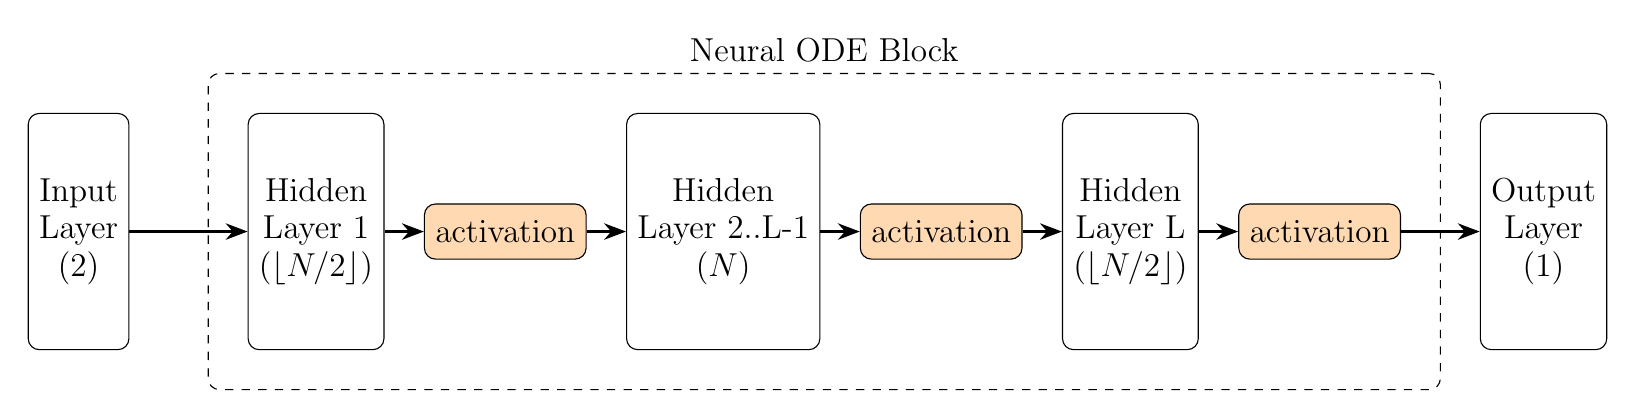
\begin{tikzpicture}[
    neuron/.style={circle, draw, minimum size=0.5cm},
    layer/.style={rectangle, draw, minimum height=3cm, rounded corners, align=center},
    arrow/.style={-{Stealth[scale=1.2]}, thick},
    activation/.style={rectangle, draw, minimum height=0.7cm, minimum width=2cm, rounded corners, fill=orange!30},
    node distance=1.5cm
    ]

    % Define the layers
    \node[layer, minimum width=1.2cm] (input) {Input\\Layer\\(2)};
    \node[layer, minimum width=1.2cm, right=of input] (h1) {Hidden\\Layer 1\\($\lfloor N/2 \rfloor$)};
    \node[activation, right=0.5cm of h1] (act1) {activation};
    \node[layer, minimum width=1.2cm, right=0.5cm of act1] (h2) {Hidden\\Layer 2..L-1\\($N$)};
    \node[activation, right=0.5cm of h2] (act2) {activation};
    \node[layer, minimum width=1.2cm, right=0.5cm of act2] (h3) {Hidden\\Layer L\\($\lfloor N/2 \rfloor$)};
    \node[activation, right=0.5cm of h3] (act3) {activation};


    \node[layer, minimum width=1.2cm, right=1cm of act3] (output) {Output\\Layer\\(1)};

    % Connect the layers
    \draw[arrow] (input) -- (h1) node[midway, above] {};
    \draw[arrow] (h1) -- (act1);
    \draw[arrow] (act1) -- (h2) node[midway, above] {};
    \draw[arrow] (h2) -- (act2);
    \draw[arrow] (act2) -- (h3) node[midway, above] {};
    \draw[arrow] (h3) -- (act3);
    \draw[arrow] (act3) -- (output) node[midway, above] {};

    % \draw[arrow] (act3) -- (h4) node[midway, above] {};
    % \draw[arrow] (h4) -- (act4);
    % \draw[arrow] (act4) -- (h5) node[midway, above] {};
    % \draw[arrow] (h5) -- (act6) node[midway, above] {};

    % \draw[arrow] (act6) -- (output) node[midway, above] {};

    % Add ODE block annotation
    \node[draw, dashed, rounded corners, fit={(h1) (h2) (h3)  (act1) (act2) (act3)}, inner sep=0.5cm, label=above:Neural ODE Block] {};

    % Add title
    % \node[above=0.7cm of input, font=\Large\bfseries, anchor=west] {Neural ODE Network Architecture};


\end{tikzpicture}

    }
    \caption{Architecture of the feedforward neural network used within the Neural ODE framework for memristor dynamics modeling. The network consists of an input layer receiving two inputs, multiple hidden layers with decreasing-increasing-decreasing neuron counts (N//2, N, N//2), activation functions between layers, and a single output. The Neural ODE block encompasses the core computational layers that approximate the derivative function $f(\xw(t), \ua(t))$ in the differential equation system.}

    \label{fig:nn-arch}
\end{figure}


\subsection{MMS Model — Mean Metastable Switch}

To evaluate the effectiveness of the proposed model, it was compared with the deterministic Mean Metastable Switch (MMS) model introduced in~\cite{Molter2016, Ostrovskii2021}. This model describes the memristor dynamics using Eq.~\eqref{eq:mms}.


\begin{align}
    \label{eq:mms}
    \dert{x} & =  \frac{1}{\tau} \Bigg( \frac{1}{1+e^{-\beta \big(\ua(t)-\von\big)}} (1-x)  -\Bigg(1- \frac{1}{1+e^{-\beta \big(\ua(t)-\voff\big)}} \Bigg) x \Bigg)
    % \beta    & = \frac{q}{kT}
\end{align}
where $\beta= \frac{q}{kT}$ is a temperature-related parameter, $\von$ denotes the switching voltage to the low-resistance state (LRS), $\voff$ denotes the switching voltage to the high-resistance state (HRS), $k$ is the Boltzmann constant, $T$ is the absolute temperature, and $q$ represents the elementary charge. The instantaneous conductance of the memristor is defined as in Eq.~\eqref{eq:conductance}.

Other conductance functions reported in the literature include, among others:
\begin{itemize}
    \item $\G_m(x) = \left( x R_{\mathrm{ON}} + (1 - x) R_{\mathrm{OFF}} \right)^{-1}$
    \item $\G_m(x) = \frac{1}{R_{\mathrm{ON}}} \left( \frac{R_{\mathrm{OFF}}}{R_{\mathrm{ON}}} \right)^{x-1}$
\end{itemize}

The influence of these functions on the memristor resistance is illustrated in Fig.~\ref{fig:m-x}.

\begin{figure}[H]
    \centering
    \resizebox{0.5\linewidth}{!}{%
        
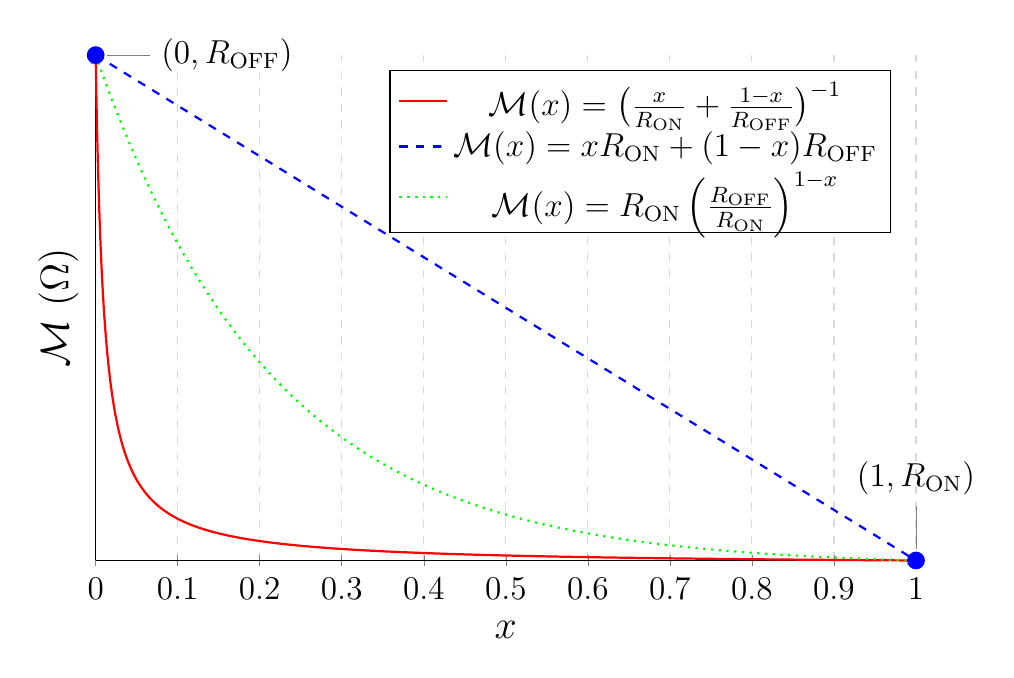
\begin{tikzpicture}
  \begin{axis}[
      width=12cm,
      height=8cm,
      xlabel={$x$},
      ylabel={ $\M$ ($\Omega$)},
      grid=major,
      grid style={dashed, gray!30},
      % xmin=0, xmax=1,
      % ymin=0, ymax=12,
      legend pos=north east,
      axis lines=left,
      tick label style={font=\normalsize},
      label style={font=\Large},
      title style={font=\Large\bfseries},
      ytick=\empty,
      clip=false
    ]

    % Define parameters
    \pgfmathsetmacro{\RON}{100}     % R_ON in ohms
    \pgfmathsetmacro{\ROFF}{10000}  % R_OFF in ohms

    % Plot the function G_m(w) = w/R_ON + (1-w)/R_OFF
    \addplot[
      domain=0:1,
      samples=1000,
      thick,
      red,
      smooth
    ] {1/(x/\RON + (1-x)/\ROFF)};


    \addlegendentry{$\M(x) = \big(\frac{x}{R_{\mathrm{ON}}} + \frac{1-x}{R_{\mathrm{OFF}}}\big)^{-1}$}

    \addplot[
      domain=0:1,
      samples=1000,
      thick,
      blue,
      smooth,
      dashed
    ] {x*\RON + (1-x)*\ROFF};


    \addlegendentry{$\M(x) = x R_{\mathrm{ON}} + (1-x) R_{\mathrm{OFF}}$}



    \addplot[
      domain=0:1,
      samples=1000,
      thick,
      green,
      smooth,
      dotted
    ] {\RON * (\ROFF/\RON)^(1-x)};

    \addlegendentry{$\M(x) = R_{\mathrm{ON}} \left( \frac{R_{\mathrm{OFF}}}{R_{\mathrm{ON}}} \right)^{1-x}$}




    % Add parameter annotations
    % \node[anchor=north west] at (axis cs:0.05,11) {
    %   \begin{tabular}{l}
    %     $R_{\mathrm{ON}} = 100\,\Omega$ \\
    %     $R_{\mathrm{OFF}} = 10000\,\Omega$
    %   \end{tabular}
    % };

    % Mark key points
    \addplot[only marks, mark=*, mark size=3pt, blue] coordinates {(0, {\ROFF}) (1, {\RON})};

    % Add labels for key points
    \node[pin=-0:{$(0, R_{\mathrm{OFF}})$}] at (axis cs:0,{\ROFF}) {};
    \node[pin=90:{$(1, R_{\mathrm{ON}})$}] at (axis cs:1,{\RON}) {};

  \end{axis}
\end{tikzpicture}
    }
    \caption{Comparison of the memristor resistance functions $R_m(x)$ for different memristor models.}
    \label{fig:m-x}
\end{figure}

In \cite{Molter2016}, the authors also proposed the Generalized Mean Metastable Switch (GMMS) model, which represents the memristor as a parallel connection of two memristors along with a Schottky diode. This model is more complex and accounts for the nonlinear current-voltage characteristics, allowing for a more accurate representation of the real memristor behavior under various operating conditions.

However, the introduction of additional parameters and nonlinearities makes this model more complicated and challenging to optimize. The derivative of the state variable corresponds to Eq.~\eqref{eq:mms}, while the current-voltage relationship is described by the following equations:

\begin{align}
    i(t)      & = \phi i_m(v, t) + (1-\phi) i_d(v)                 \\
    i_d(v)    & = \alpha_f e^{\beta_f v} - \alpha_r e^{-\beta_r v} \\
    i_m(v, t) & = \G_m(x) v
\end{align}

where $\phi \in [0,1]$ is a parameter representing the fraction of the total current flowing through the memristor relative to the entire current through the device. The parameters $\alpha_f$, $\beta_f$, $\alpha_r$, and $\beta_r$ are positive constants characterizing the forward and reverse current behavior along the Schottky barrier.


In the case of the GMMS model, an additional challenge arises due to the Schottky effect, which introduces nonlinearity into the current–voltage characteristic. When the memristor is connected in series with a resistor, this requires solving a nonlinear equation of the form Eq. \eqref{eq:nonlinear_eq} numerically at each time step. As a result, the system of ordinary differential equations is transformed into a differential-algebraic equation (DAE).
\begin{equation}
    v_s(t) = v_r(t) + v_m(t)
    \label{eq:nonlinear_eq}
\end{equation}
where $v_s(t)$ denotes the supply voltage, $v_r(t) = R_s i(t)$ is the voltage across the resistor, and $v_m(t)$ is the voltage across the memristor.

This formulation renders the system stiff and prevents the straightforward application of automatic differentiation with respect to model parameters in the objective function. An alternative approach to address this is the use of implicit differentiation.
Let $F$ be a function defined by the equation:
\begin{equation}
    F(v_m, t) = v_s(t) - v_r(v_m, t) - v_m(t) = 0.
\end{equation}
Applying the chain rule yields:
\begin{equation}
    \frac{\mathrm{d} F}{\mathrm{d} t} = \frac{\partial F}{\partial v_m} \frac{\mathrm{d} v_m}{\mathrm{d} t} + \frac{\partial F}{\partial t} = 0,
\end{equation}
which implies:
\begin{equation}
    \frac{\mathrm{d} v_m}{\mathrm{d} t} = - \frac{\partial F / \partial t}{\partial F / \partial v_m}.
\end{equation}
Substituting the expressions gives:
\begin{equation}
    \frac{\mathrm{d} v_m}{\mathrm{d} t} = - \frac{\mathrm{d} v_s}{\mathrm{d} t} \cdot \frac{1}{ - R_s \left( \G_{m} \phi + (1 - \phi) \left( \alpha_f \beta_f e^{\beta_f v_m} + \alpha_r \beta_r e^{-\beta_r v_m} \right) \right) - 1 }.
\end{equation}

Thus, the system requires an additional state variable; however, it is not necessary to solve a nonlinear system of equations at each time step. Consequently, the system of differential equations describing the memristor-resistor setup using the GMMS model is as follows:

\begin{equation}
    \begin{cases}
        \displaystyle \frac{\mathrm{d} x}{\mathrm{d} t} = \frac{1}{\tau} \left( \frac{1}{1 + e^{-\beta \left(v_m(t) - v_{\mathrm{on}}\right)}} (1 - x) - \left( 1 - \frac{1}{1 + e^{-\beta \left(v_m(t) - v_{\mathrm{off}}\right)}} \right) x \right), \\
        \displaystyle \frac{\mathrm{d} v_m}{\mathrm{d} t} = \frac{\mathrm{d} v_s}{\mathrm{d} t} \cdot \frac{1}{R_s \left( \G_{m} \phi + (1 - \phi) \left( \alpha_f \beta_f e^{\beta_f v_m} + \alpha_r \beta_r e^{-\beta_r v_m} \right) \right) - 1}.
    \end{cases}
\end{equation}


\subsection{Objective Function}

The loss function based on the phase portrait is designed to simultaneously account for both the absolute signal magnitudes and its dynamic structure. To this end, it is defined as the sum of four components, each serving a distinct and complementary role in the optimization process. The total loss function is given by:

\begin{equation}
    \mathcal{L}_{\mathrm{total}} = \lambda_{\mathrm{base}} \cdot \mathcal{L}_{\mathrm{base}} + \lambda_{\mathrm{vel}} \cdot \mathcal{L}_{v} + \lambda_{\mathrm{curv}} \cdot \mathcal{L}_{c} + \lambda_{\mathrm{iv}} \cdot \mathcal{L}_{\mathrm{iv}} +\sum^{N_c}_{i=1} \lambda_{\mathrm{con}_i} \cdot \mathcal{L}_{\mathrm{con}_i}(x),
    \label{eq:loss_function}
\end{equation}

Here, $\mathcal{L}_{\mathrm{base}}$ denotes the primary error term,  measuring the difference between predicted and reference values, in that case the mean squared error (MSE). The term $\mathcal{L}_{v}$ enforces accurate modeling of the velocity characteristics by considering the derivatives of trajectories in phase space. The component $\mathcal{L}_{c}$ promotes consistency of the trajectories in terms of their curvature, for example by analyzing changes in trajectory direction or curvature.
Component $\mathcal{L}_{\mathrm{iv}}$ focuses on the $i_m-v_m$ relationship, ensuring that the current-voltage characteristics are accurately captured. Finally, $\mathcal{L}_{\mathrm{con}}(x)$ introduces additional physical or structural constraints that the model is required to satisfy, including conditions of stability, nonlinearities, or conformity to the underlying physical model. The weighting coefficients $\lambda_{\mathrm{base}}$, $\lambda_{\mathrm{vel}}$, $\lambda_{\mathrm{curv}}$, and $\lambda_{\mathrm{iv}}$ balance the influence of each term within the overall loss function according to the priorities of the modeling task, and each of the values were calculated during optimization using the Geometric Loss Strategy (GLS) with the following algorithm presented in Algorithm~\ref{alg:adaptive_loss_balancing}.

\begin{algorithm}[H]
    \caption{Adaptive Loss Balancing with Clamping}
    \label{alg:adaptive_loss_balancing}
    \begin{algorithmic}[1]
        \Require Loss terms $L_{\text{base}}, L_{\text{vel}}, L_{\text{curv}}, L_{\text{iv}}$, small constant $\varepsilon > 0$, clamp bounds $[\lambda_{\min}, \lambda_{\max}]$
        \Ensure Adaptive weights $\lambda_{\text{base}}, \lambda_{\text{vel}}, \lambda_{\text{curv}}, \lambda_{\text{iv}}$
        \Statex

        \State Collect losses:
        \[
            \mathbf{L} \gets [L_{\text{base}}, L_{\text{vel}}, L_{\text{curv}}, L_{\text{iv}}]
        \]

        \State Compute geometric mean:
        \[
            \overline{L}_{\text{geo}} \gets \exp\!\left(\frac{1}{|\mathbf{L}|} \sum_{i=1}^{|\mathbf{L}|} \ln(L_i + \varepsilon)\right)
        \]

        \For{each loss $L_i \in \mathbf{L}$}
        \State Compute raw weight:
        \[
            \lambda_i \gets \frac{\overline{L}_{\text{geo}}}{L_i + \varepsilon}
        \]
        \State Clamp weight:
        \[
            \lambda_i \gets \min\!\big(\max(\lambda_i, \, \lambda_{\min}), \, \lambda_{\max}\big)
        \]
        \EndFor

        \State Return weights $(\lambda_{\text{base}}, \lambda_{\text{vel}}, \lambda_{\text{curv}}, \lambda_{\text{iv}})$
    \end{algorithmic}
\end{algorithm}


For circuit trajectory datasets indexed by $k = 1, \ldots, N_{\text{traj}}$, a trajectory-specific standardization procedure is implemented to normalize each electrical variable $z \in \{v, i\}$ (representing voltage and current measurements, respectively). This normalization process utilizes the standard deviation computed independently for each individual trajectory sequence, ensuring statistical consistency within each temporal dataset.

The trajectory-specific standard deviation is calculated using the unbiased sample estimator:
\begin{equation}
    \sigma_{z,k} = \sqrt{\frac{1}{T-1} \sum_{t=1}^{T} \left(z_{k,t}^{\mathrm{true}} - \bar{z}_k^{\mathrm{true}}\right)^2}
\end{equation}

where the trajectory-specific temporal mean is defined as:
\begin{equation}
    \bar{z}_k^{\mathrm{true}} = \frac{1}{T} \sum_{t=1}^{T} z_{k,t}^{\mathrm{true}}
\end{equation}

The parameter $T$ represents the temporal resolution of the trajectory, corresponding to the total number of discrete time-series sampling points within each measurement sequence.

This trajectory-wise normalization methodology serves several critical analytical objectives in circuit analysis and machine learning applications. Primarily, it establishes scale invariance across electrical signals exhibiting disparate amplitude characteristics, thereby facilitating quantitative comparison of dynamic waveform morphologies independent of absolute magnitude variations. Furthermore, this standardization approach enhances the numerical stability and convergence properties of optimization algorithms employed in neural network training procedures.

By implementing trajectory-specific normalization rather than global standardization, the methodology preserves the inherent temporal dynamics and statistical properties unique to each circuit configuration while simultaneously ensuring that amplitude disparities do not introduce systematic bias during pattern recognition, feature extraction, or predictive modeling procedures. This approach is particularly advantageous in scenarios involving heterogeneous circuit topologies or varying operational conditions, where maintaining the relative temporal structure of electrical phenomena is paramount for accurate system identification and dynamic analysis.
The neural network loss function comprises several specialized components designed to optimize memristor circuit modeling performance across multiple dynamical characteristics. Each component addresses specific aspects of the temporal and nonlinear behavior exhibited by memristive systems.

The fundamental component of the loss function is responsible for model fitting to experimental voltage-current data, incorporating trajectory-specific normalization procedures. This component minimizes the mean squared error (MSE) between predicted and ground-truth voltage and current waveforms, normalized by the standard deviation of each individual trajectory. This normalization ensures scale invariance across datasets with varying amplitude characteristics.The mean squared error for a sequence of $n$ data points is defined in Eq~\eqref{eq:mse}:
\begin{equation}
    \mathrm{MSE}(\hat{y}, y) = \frac{1}{n} \sum_{i=1}^{n} (\hat{y}_i - y_i)^2
    \label{eq:mse}
\end{equation}
where $\hat{y}_i$ represents the predicted values and $y_i$ represents the true values.

The base loss is formally expressed as it shown in Eq.~\eqref{eq:base_loss}:
\begin{equation}
    \mathcal{L}_{\mathrm{base}} = \frac{1}{N_{\text{traj}}} \sum_{k=1}^{N_{\text{traj}}} \left[\mathrm{MSE}\left(\frac{v_{\mathrm{pred},k}}{\sigma_{v,k}}, \frac{v_{\mathrm{true},k}}{\sigma_{v,k}}\right) +  \mathrm{MSE}\left(\frac{i_{\mathrm{pred},k}}{\sigma_{i,k}}, \frac{i_{\mathrm{true},k}}{\sigma_{i,k}}\right)\right]
    \label{eq:base_loss}
\end{equation}
where $v_{\mathrm{pred},k}$ and $i_{\mathrm{pred},k}$ represent the predicted voltage and current for trajectory $k$, while $v_{\mathrm{true},k}$ and $i_{\mathrm{true},k}$ denote the corresponding experimental measurements.

The first-order dynamics comparison enables evaluation of temporal derivative agreement between model predictions and experimental data, particularly critical for capturing rapid memristor state transitions. This component ensures that the neural network learns not only absolute signal values but also their instantaneous rates of change, which is fundamental for accurate modeling of dynamic systems exhibiting switching phenomena. The first-order loss component is defined as:
\begin{equation}
    \mathcal{L}_{v} = \frac{1}{N_{\text{traj}}} \sum_{k=1}^{N_{\text{traj}}} \left[
        \mathrm{MSE}\left(\frac{\tfrac{\mathrm{d}v}{\mathrm{d}t}_{\mathrm{pred},k}}{\sigma_{\dot{v},k}}, \frac{\tfrac{\mathrm{d}v}{\mathrm{d}t}_{\mathrm{true},k}}{\sigma_{\dot{v},k}}\right) +
        \mathrm{MSE}\left(\frac{\tfrac{\mathrm{d}i}{\mathrm{d}t}_{\mathrm{pred},k}}{\sigma_{\dot{i},k}}, \frac{\tfrac{\mathrm{d}i}{\mathrm{d}t}_{\mathrm{true},k}}{\sigma_{\dot{i},k}}\right)
        \right]
    \label{eq:loss_v}
\end{equation}

This formulation captures the velocity characteristics of electrical variables, ensuring that transient behaviors and switching dynamics are accurately reproduced by the model.

The second-order comparison term addresses trajectory curvature characteristics, which are essential for capturing subtle variations in system dynamics that manifest as nonlinear memristor behaviors. This component facilitates superior representation of curvature properties within the phase-space trajectory, particularly important for modeling systems exhibiting complex nonlinear and highly dynamic responses. The curvature loss is formulated as:
\begin{equation}
    \mathcal{L}_{c} = \frac{1}{N_{\text{traj}}} \sum_{k=1}^{N_{\text{traj}}} \left[
        \mathrm{MSE}\left(\frac{\tfrac{\mathrm{d}^2 v}{\mathrm{d}t^2}_{\mathrm{pred},k}}{\sigma_{\ddot{v},k}}, \frac{\tfrac{\mathrm{d}^2 v}{\mathrm{d}t^2}_{\mathrm{true},k}}{\sigma_{\ddot{v},k}}\right) +
        \mathrm{MSE}\left(\frac{\tfrac{\mathrm{d}^2 i}{\mathrm{d}t^2}_{\mathrm{pred},k}}{\sigma_{\ddot{i},k}}, \frac{\tfrac{\mathrm{d}^2 i}{\mathrm{d}t^2}_{\mathrm{true},k}}{\sigma_{\ddot{i},k}}\right)
        \right]
    \label{eq:loss_c}
\end{equation}

By incorporating second-order temporal derivatives, this component ensures that acceleration characteristics and higher-order dynamical features are preserved during the learning process.

The $v_m-i_m$ relationship is crucial for accurately capturing the interplay between voltage and current in memristive systems, the computation pseudocode for this component is as presented in Algorithm~\ref{alg:vm_im_relationship}.

\begin{algorithm}[H]
    \caption{$v-i$ Curve Loss Computation}
    \label{alg:vm_im_relationship}
    \begin{algorithmic}[1]
        \Require True voltages $\mathbf{v}_{\text{true}} \in \mathbb{R}^{B \times N}$, true currents $\mathbf{i}_{\text{true}}$, predicted currents $\mathbf{i}_{\text{pred}}$
        \Ensure $v - i$ loss $\mathcal{L}_{\text{vi}}$
        \Statex

        \For{each batch element $b = 1, \dots, B$}
        \State Sort voltages: $v_{\text{sorted}} \gets \text{sort}(v_{\text{true},b})$
        \State Get sorting indices: $v_{\text{indices}}$
        \State Reorder currents according to voltage order:
        \[
            i_{\text{sorted}}^{\text{true}} \gets i_{\text{true},b}[v_{\text{indices}}]
        \]
        \[
            i_{\text{sorted}}^{\text{pred}} \gets i_{\text{pred},b}[v_{\text{indices}}]
        \]
        \EndFor

        \State Compute mean squared error:
        \[
            \mathcal{L}_{\text{vi}} \gets \frac{1}{B N} \sum_{b=1}^{B} \sum_{j=1}^{N}
            \left( i_{\text{sorted},b}^{\text{pred},(j)} - i_{\text{sorted},b}^{\text{true},(j)} \right)^2
        \]

        \State \Return $\mathcal{L}_{\text{IV}}$
    \end{algorithmic}
\end{algorithm}
To enforce parameter bounds within specified intervals, a sophisticated constraint loss function utilizing smooth sigmoid transitions is implemented. This component prevents parameter drift beyond physically meaningful ranges while maintaining differentiability for gradient-based optimization algorithms. The constraint loss is mathematically expressed as:
% \begin{equation}
%     \mathcal{L}_{\mathrm{con}}(\mathbf{x}) =  \mathbb{E}\left[\left(
%         \sigma\left(-\frac{\mathbf{x} - (a + \delta)}{\delta/4}\right) \cdot ((a + \delta) - \mathbf{x}) +
%         \sigma\left(\frac{\mathbf{x} - (b - \delta)}{\delta/4}\right) \cdot (\mathbf{x} - (b - \delta))
%         \right)^2\right]
% \end{equation}

% where the constituent parameters are defined as follows:
% \begin{itemize}
%     \item $\sigma(z) = \frac{1}{1 + e^{-z}}$ represents the sigmoid activation function
%     \item $a$ and $b$ denote the lower and upper bounds of the admissible parameter range, respectively
%     \item $\delta$ specifies the transition margin (width of the transitional zone between admissible and penalized parameter regions)
%     \item $\lambda_{\mathrm{con}}$ represents the weighting coefficient controlling the constraint enforcement strength
%     \item $\mathbb{E}$ denotes the expectation operator (ensemble average over the parameter set or trajectory collection)
% \end{itemize}

\begin{equation}
    \mathcal{L_{\mathrm{con}}}(x) = \mathbb{E}\left[\left(
        \frac{1}{1 + \exp\!\left(\tfrac{x-a}{f}\right)} \cdot (a-x) \;+\;
        \frac{1}{1 + \exp\!\left(-(x-b)/f\right)} \cdot (x-b)
        \right)^{2}\right]
\end{equation}

where the constituent parameters are defined as follows:
\begin{itemize}
    \item $\sigma(z) = \tfrac{1}{1+e^{-z}}$ represents the sigmoid activation function (implicitly used)
    \item $a$ and $b$ denote the lower and upper bounds of the admissible parameter range, respectively
    \item $f$ is a smoothing (scaling) factor controlling the steepness of the transition near the bounds
    \item the term $\tfrac{1}{1+\exp((x-a)/f)}(a-x)$ penalizes values of $x$ below the lower bound $a$
    \item the term $\tfrac{1}{1+\exp(-(x-b)/f)}(x-b)$ penalizes values of $x$ above the upper bound $b$
    \item squaring ensures the penalty is non-negative and grows quadratically with the violation magnitude
    \item $\mathbb{E}[\cdot]$ denotes the expectation operator (ensemble average over samples or trajectories)
\end{itemize}


This constraint formulation provides smooth penalty gradients that guide parameters toward the feasible region while avoiding discontinuities that could disrupt the optimization process. The sigmoid-based transitions ensure that the constraint becomes progressively more restrictive as parameters approach the boundary limits, promoting stable convergence behavior.


During neural network training, specific interval constraints were implemented to ensure physically meaningful and numerically stable parameter values that align with experimental memristor characteristics and theoretical boundaries. These constraints prevent parameter drift into unphysical regimes while maintaining the differentiability required for gradient-based optimization algorithms.

The following constraint intervals were applied to critical memristor model parameters where the $\M(\xvec, v(t))$ was fixed:

\begin{itemize}
    \item $R_{\mathrm{ON}} \in (0, R_{\mathrm{OFF}})\,\mathrm{k}\Omega$ and $R_{\mathrm{OFF}} \in (R_{\mathrm{ON}}, 200)\,\mathrm{k}\Omega$ – These constraints establish a physically meaningful hierarchy where the ON-state resistance is strictly smaller than the OFF-state resistance ($R_{\mathrm{ON}} < R_{\mathrm{OFF}}$), consistent with typical memristor switching behavior. The lower bound for $R_{\mathrm{ON}}$ prevents zero resistance values that would cause numerical singularities in current calculations, while the upper bound of 200 k$\Omega$ for $R_{\mathrm{OFF}}$ reflects experimentally observed resistance ranges in memristive devices and ensures computational stability during optimization.


    \item $x_0 \in (0, 1)$ – This constraint restricts the initial internal state variable to the normalized domain, ensuring that the memristor begins operation within physically admissible boundaries. The open interval prevents boundary singularities that could occur at $x_0 = 0$ or $x_0 = 1$.

    \item $x(t) \in (0, 1)$ – This temporal constraint maintains the internal state variable within the normalized domain throughout the entire simulation duration, preserving the physical interpretation of $x(t)$ as a fractional parameter representing the extent of ionic migration or structural modification within the memristive element.
\end{itemize}

These constraints are particularly crucial for memristor modeling because they preserve the fundamental physical relationships governing resistive switching phenomena while preventing the emergence of artifacts that could arise from parameter values outside the feasible operating regime.



The operational characteristics of the constraint function $\mathcal{L}_{\mathrm{con}}(\mathbf{x})$ are illustrated in Figure~\ref{fig:constrains} for the parameter configuration: $a=0$, $b=1$, $\delta=0.01$ over the evaluation domain $\mathbf{x} \in (-0.5, 1.5)$. This visualization demonstrates the smooth sigmoid-based transition behavior that provides continuous penalty gradients while maintaining differentiability across the parameter space. The constraint function architecture ensures that parameters within the admissible range $(0,1)$.

\begin{figure}[H]
    \centering
    \resizebox{0.5\linewidth}{!}{%
        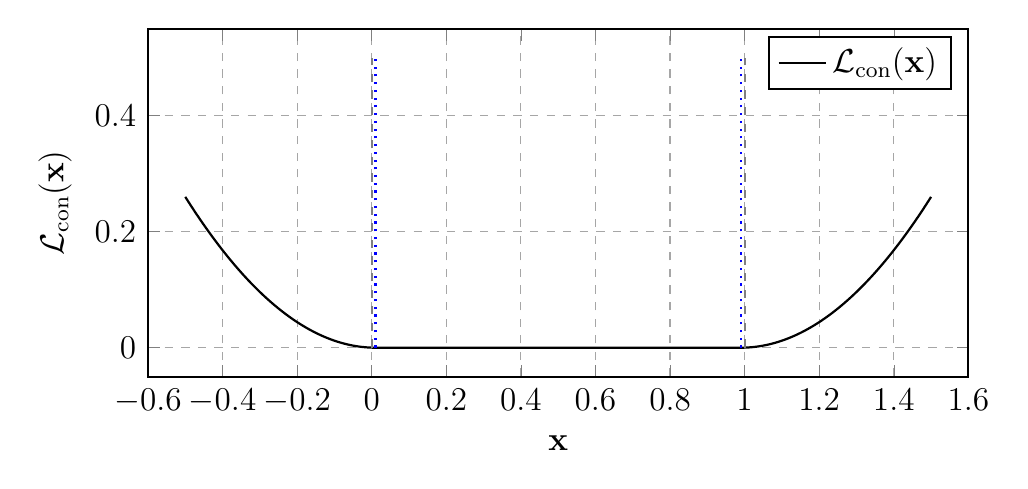
\begin{tikzpicture}
  \begin{axis}[
    width=12cm,
    height=6cm,
    xlabel={$\mathbf{x}$},
    ylabel={$\mathcal{L}_{\mathrm{con}}(\mathbf{x})$},
    grid=major,
    grid style={dashed,gray!70},
    legend style={at={(0.98,0.98)},anchor=north east},
    domain=-0.5:1.5,
    samples=500,
    thick,
    % Automatic spacing like matplotlib margins
    enlarge x limits=0.05,
    enlarge y limits=0.1,
    ]

    % Main function plot
    \addplot [
      color=black,
    ]
    {(1/(1 + exp(-(-((x - 0.01)/0.0025)))) * (0.01 - x)
      + 1/(1 + exp(-((x - 0.99)/0.0025))) * (x - 0.99))^2};
    \addlegendentry{$\mathcal{L}_{\mathrm{con}}(\mathbf{x})$}

    % Vertical reference lines using simple approach
    \addplot[dashed, gray, forget plot] coordinates {(0,0) (0,0.5)};
    \addlegendentry{$a = 0$}

    \addplot[dashed, gray, forget plot] coordinates {(1,0) (1,0.5)};
    \addlegendentry{$b = 1$}

    \addplot[dotted, blue, forget plot] coordinates {(0.01,0) (0.01,0.5)};
    \addlegendentry{$a + \delta$}

    \addplot[dotted, blue, forget plot] coordinates {(0.99,0) (0.99,0.5)};
    \addlegendentry{$b - \delta$}
  \end{axis}
\end{tikzpicture}
    }
    \caption{Operational characteristics of the constraint function $\mathcal{L}_{\mathrm{con}}(\mathbf{x})$ demonstrating smooth penalty transitions for parameter bounds $a=0$, $b=1$ with transition margin $\delta=0.01$ evaluated over the domain $\mathbf{x} \in (-0.5, 1.5)$. The function exhibits minimal penalty within the feasible region $(0,1)$ and progressively increasing penalties as parameters approach or exceed the boundary limits.}
    \label{fig:constrains}
\end{figure}



% \subsection{Impl


\section{Results}

Representative simulation results demonstrating the neural network model's predictive capabilities are presented in Figure~\ref{fig:sample-results} through comparative analysis of a tungsten-doped memristor device subjected to sinusoidal voltage excitation with an amplitude of 1V and frequency of 1Hz. These specific excitation parameters were selected to capture the characteristic switching dynamics while maintaining operation within the device's linear regime, enabling comprehensive evaluation of the model's ability to reproduce fundamental memristive behaviors.

The analysis encompasses three critical dynamic characteristics that collectively characterize memristor behavior: temporal current evolution, applied voltage profiles, and voltage-current hysteresis relationships. The temporal current response reveals the device's instantaneous electrical behavior and switching kinetics, while the applied voltage profile confirms the fidelity of the input stimulus. Most significantly, the voltage-current hysteresis loops ($v_m - i_m$) demonstrate the nonlinear relationship between these electrical quantities and illustrate the fundamental memory properties that define memristive behavior.

The hysteresis loops are particularly diagnostic of memristor performance, as their shape, area, and switching thresholds directly reflect the underlying ionic transport mechanisms and structural modifications responsible for resistive switching. The pinched hysteresis characteristic observed at the origin serves as a definitive signature of memristive behavior, while the loop area quantifies the energy dissipation associated with switching events. These features enable comprehensive validation of the neural network model's ability to capture both the static and dynamic aspects of memristor operation.

\newcommand{\subwidth}{0.32\linewidth}
\begin{figure}[H]
    \centering
    \begin{subfigure}[b]{\subwidth}
        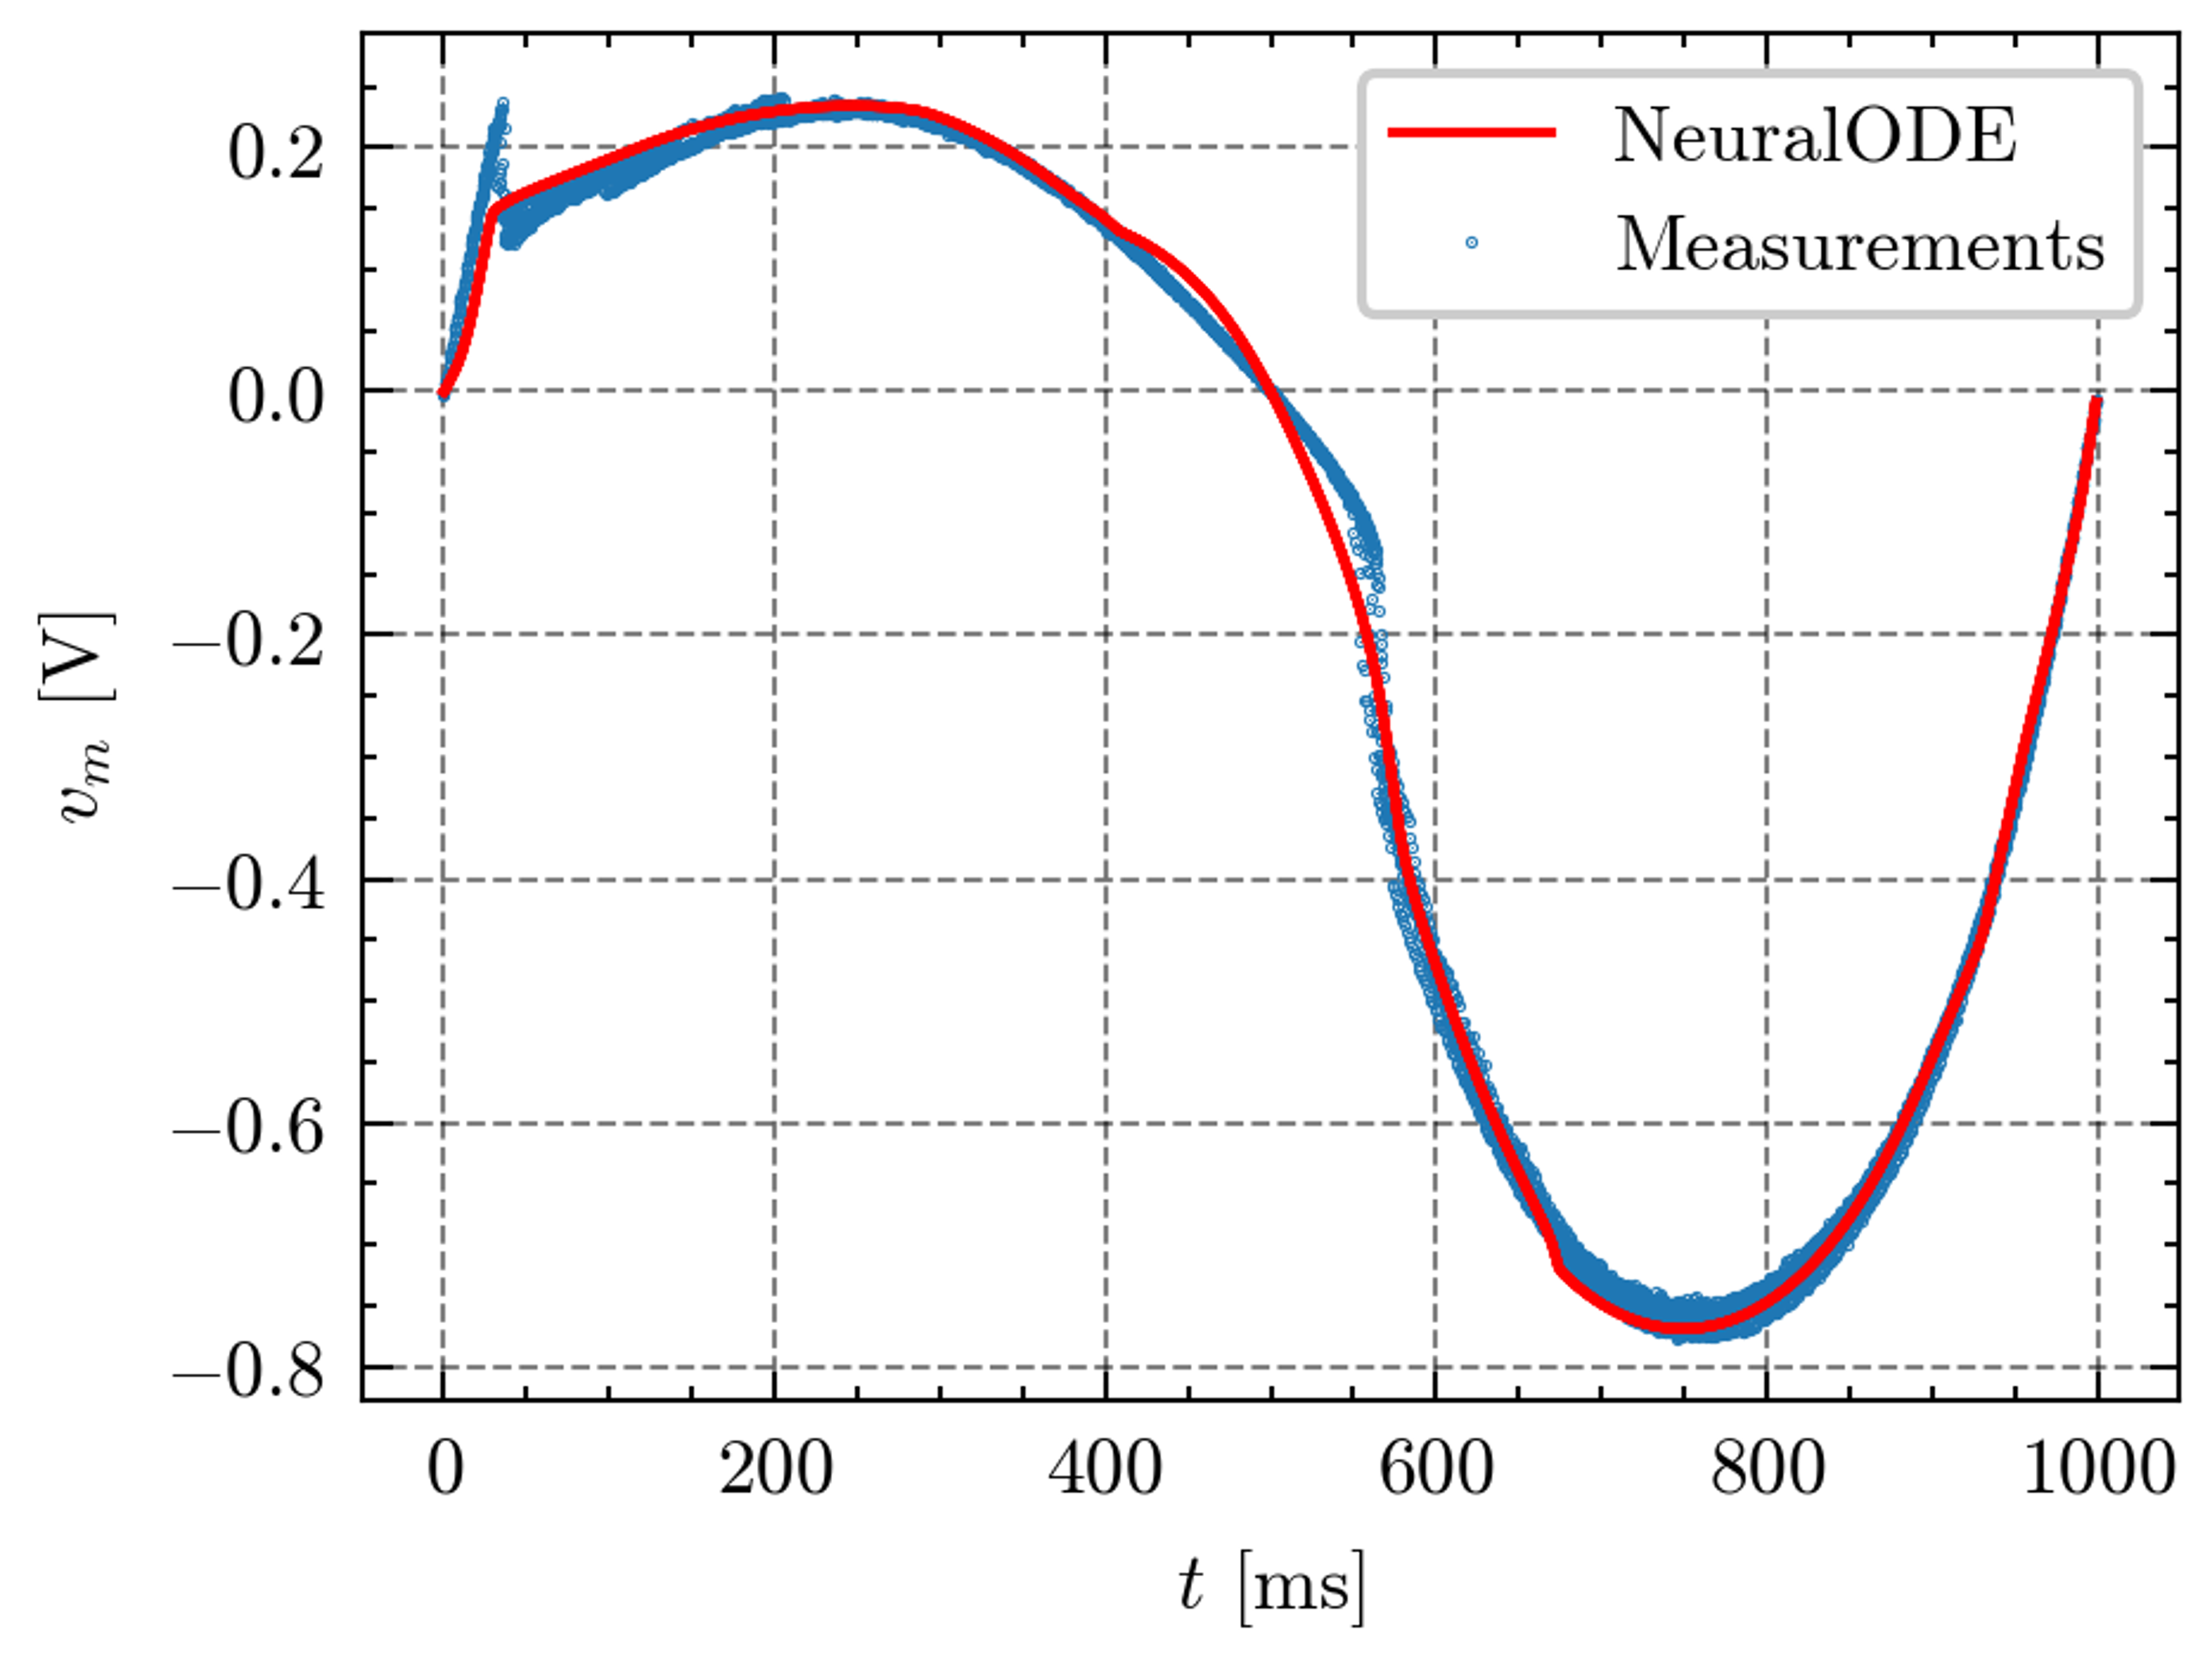
\includegraphics[width=\linewidth]{sample_results/v_m.png}
        \caption{Applied voltage waveform}
    \end{subfigure}
    % \hfill
    \begin{subfigure}[b]{\subwidth}
        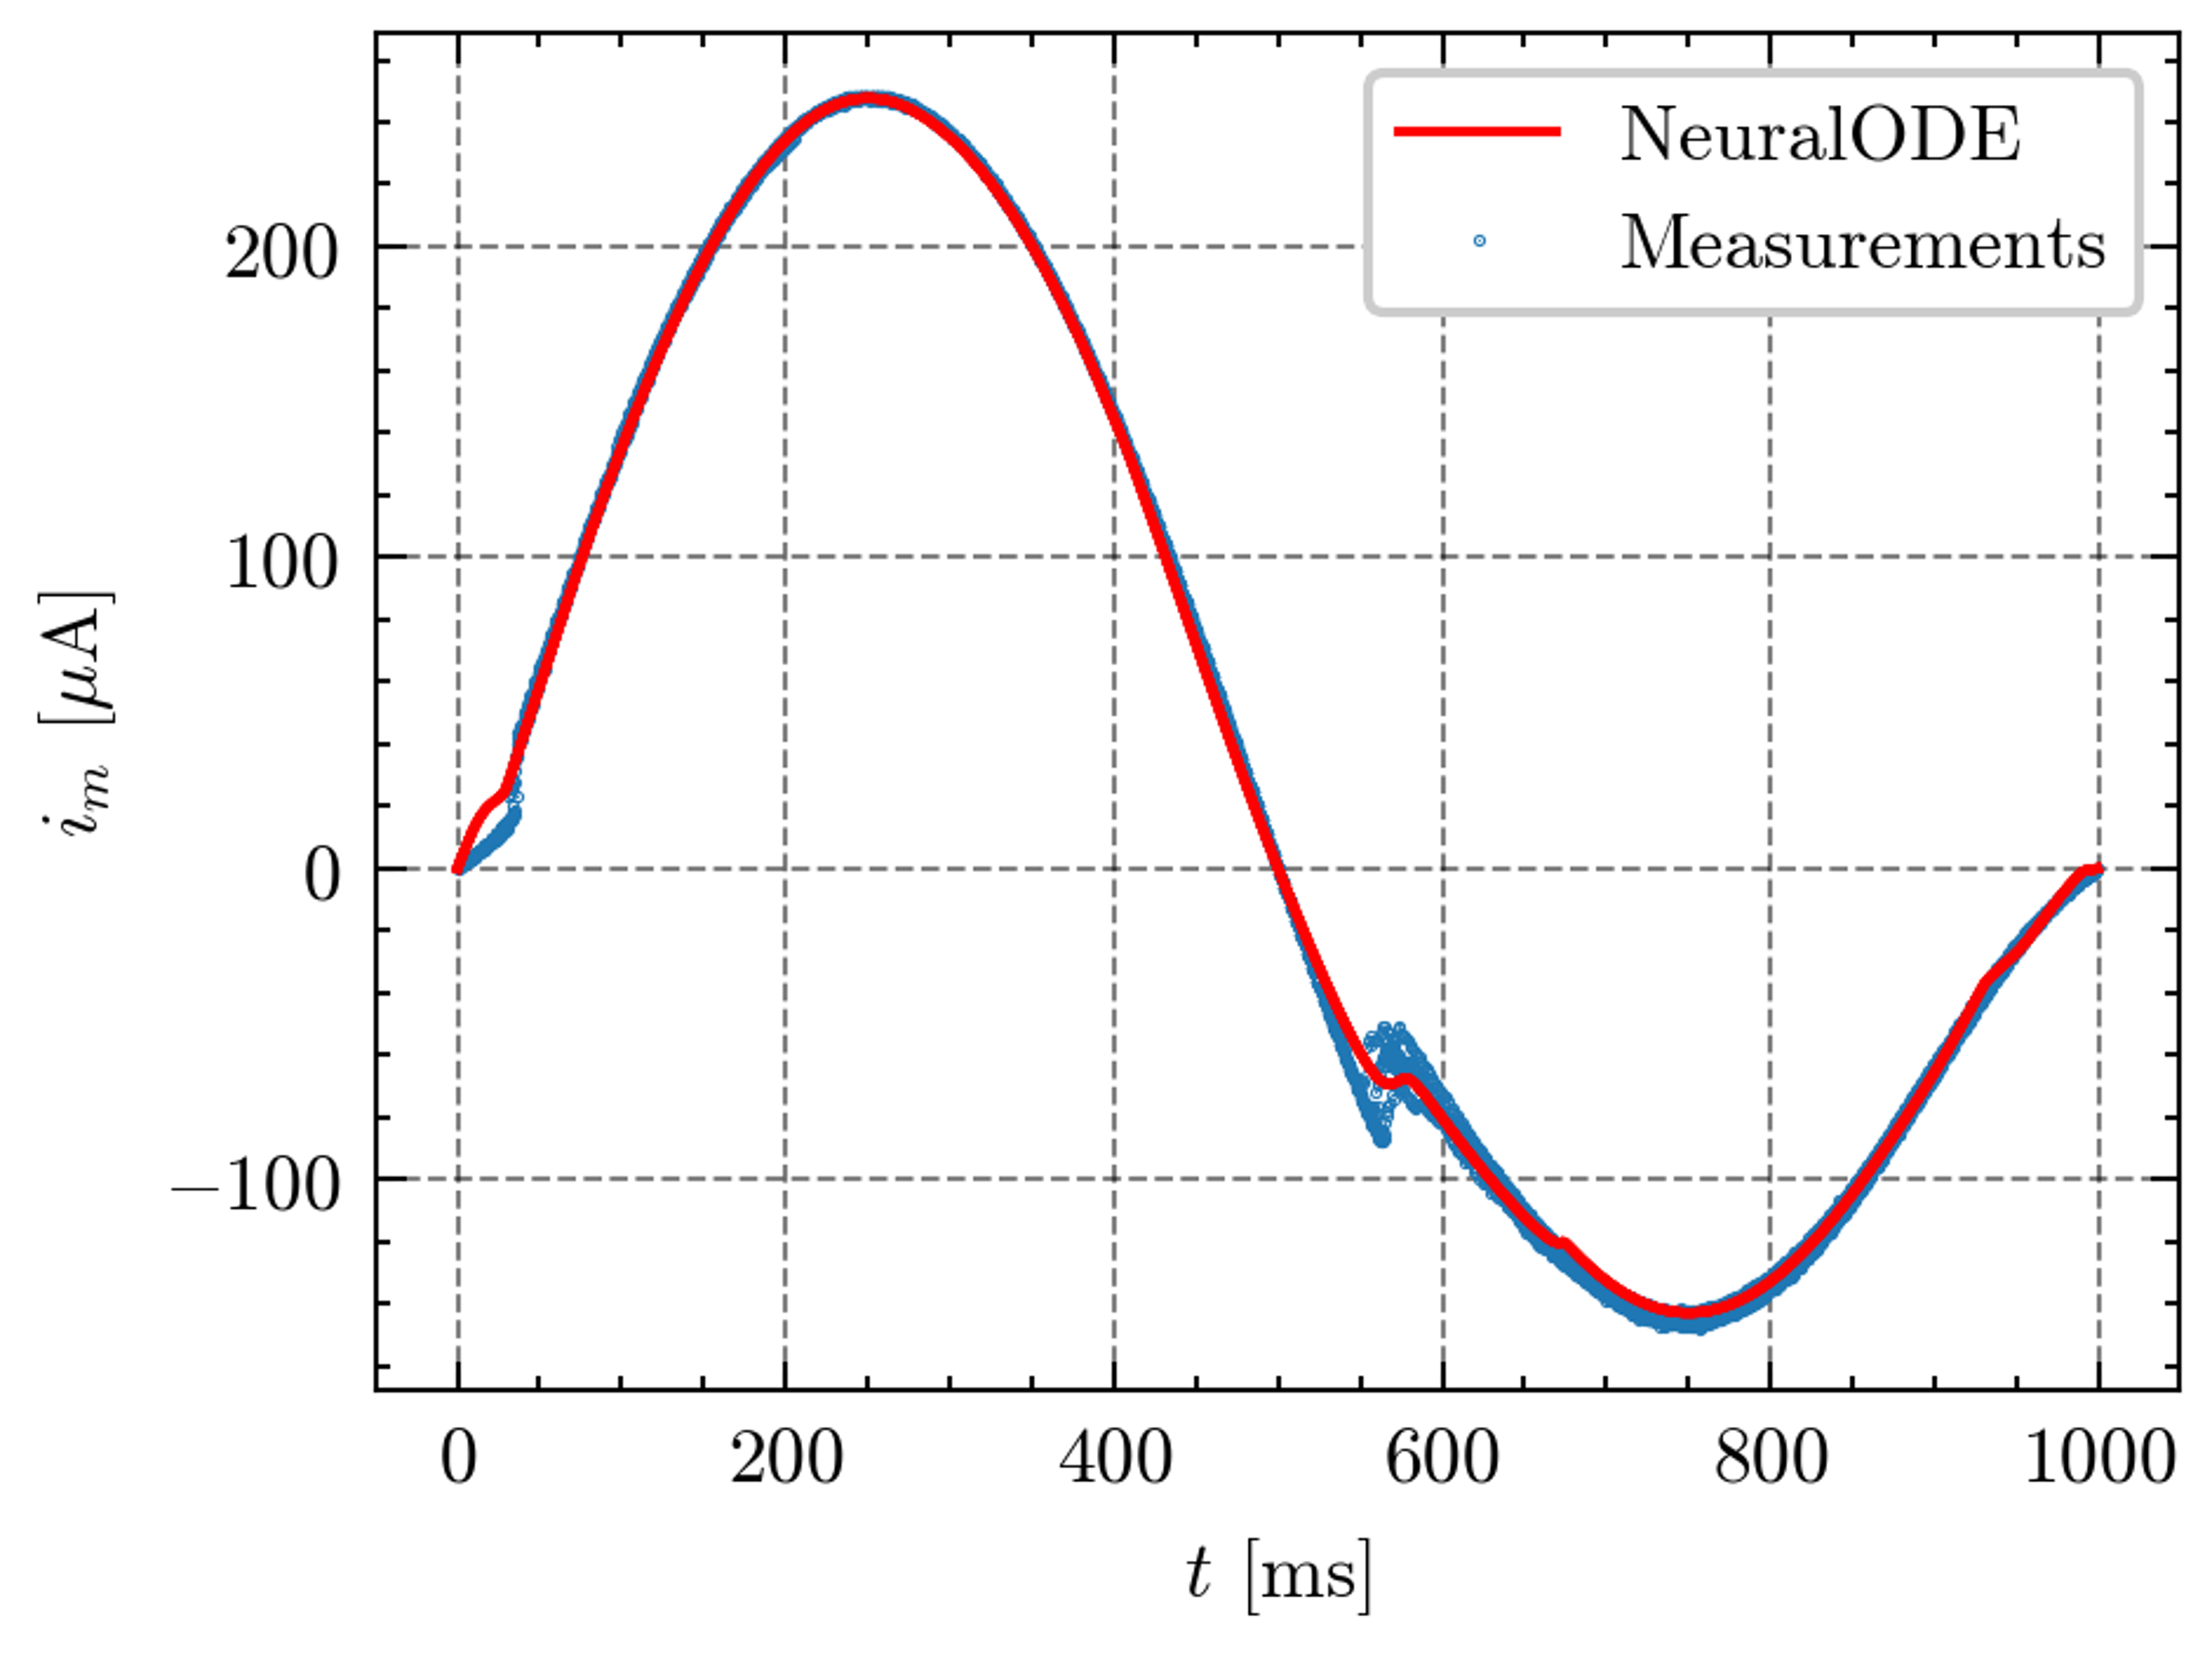
\includegraphics[width=\linewidth]{sample_results/i_m.png}
        \caption{Memristor current response}
    \end{subfigure}
    \begin{subfigure}[b]{\subwidth}
        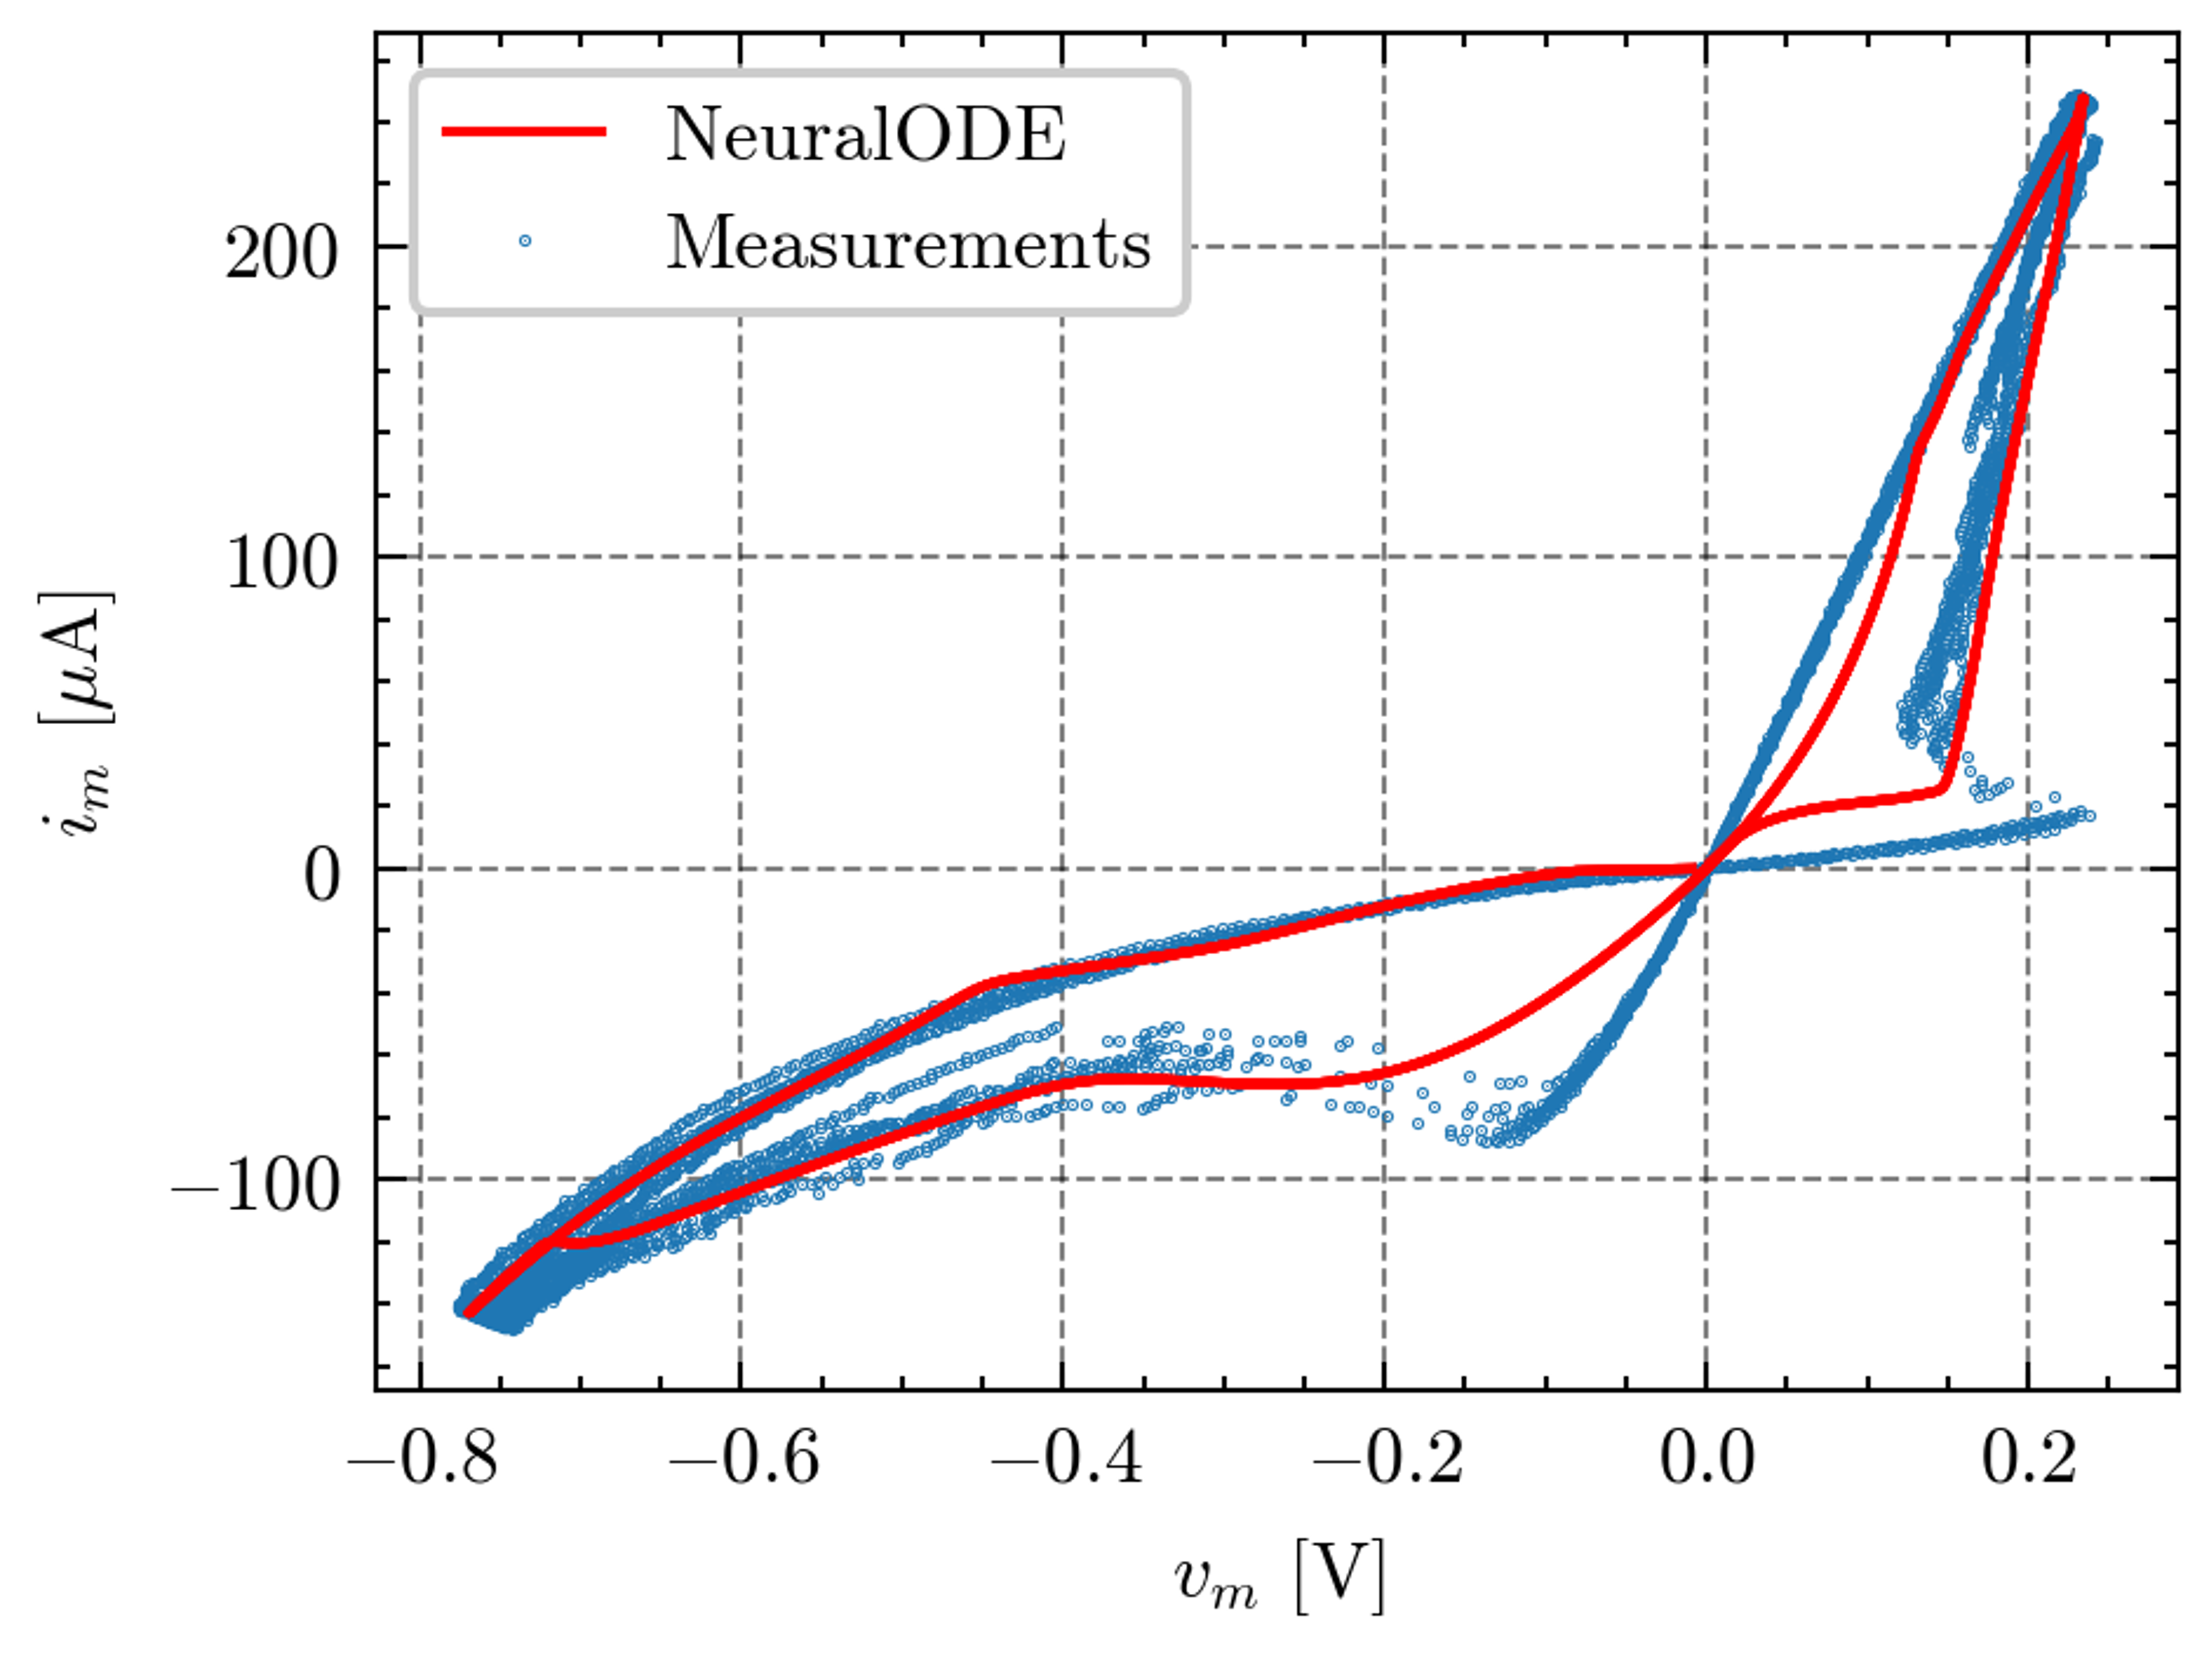
\includegraphics[width=\linewidth]{sample_results/hysteresis.png}
        \caption{Voltage-current hysteresis characteristic}
    \end{subfigure}
    \caption{Representative simulation results for tungsten-doped memristor dynamics under sinusoidal voltage excitation (amplitude: 1V, frequency: 1Hz). (a) Applied voltage waveform demonstrating the sinusoidal input stimulus, (b) Predicted memristor current response showing nonlinear temporal evolution and switching characteristics, (c) Voltage-current hysteresis loop ($v_m - i_m$) illustrating the characteristic pinched behavior and memory properties fundamental to memristive operation. The neural network model successfully captures the essential features of memristor dynamics including switching thresholds, nonlinear conductance modulation, and hysteretic memory effects.}
    \label{fig:sample-results}
\end{figure}

% \subsection{Zagregowane wyniki dla różnych architektur sieci neuronowej}

\subsection{Aggregated Results for Neural Network Architecture Comparison}

To systematically evaluate the impact of neural network architectural choices on memristor modeling accuracy, a comprehensive comparison was conducted across multiple network configurations. This analysis employed period-averaged waveforms to eliminate temporal phase variations and focus on the fundamental characteristics of memristive behavior reproduction. The period-averaging methodology involves temporal alignment of multiple excitation cycles followed by ensemble averaging, which effectively suppresses transient artifacts and highlights the steady-state dynamical properties captured by each architecture.

The architectural comparison encompasses variations in both network depth (number of hidden layers) and width (neurons per layer), enabling systematic investigation of the representational capacity required for accurate memristor dynamics modeling. This analysis is crucial for determining optimal network complexity that balances modeling accuracy with computational efficiency and training stability.

\begin{figure}[htbp!]
    \centering
    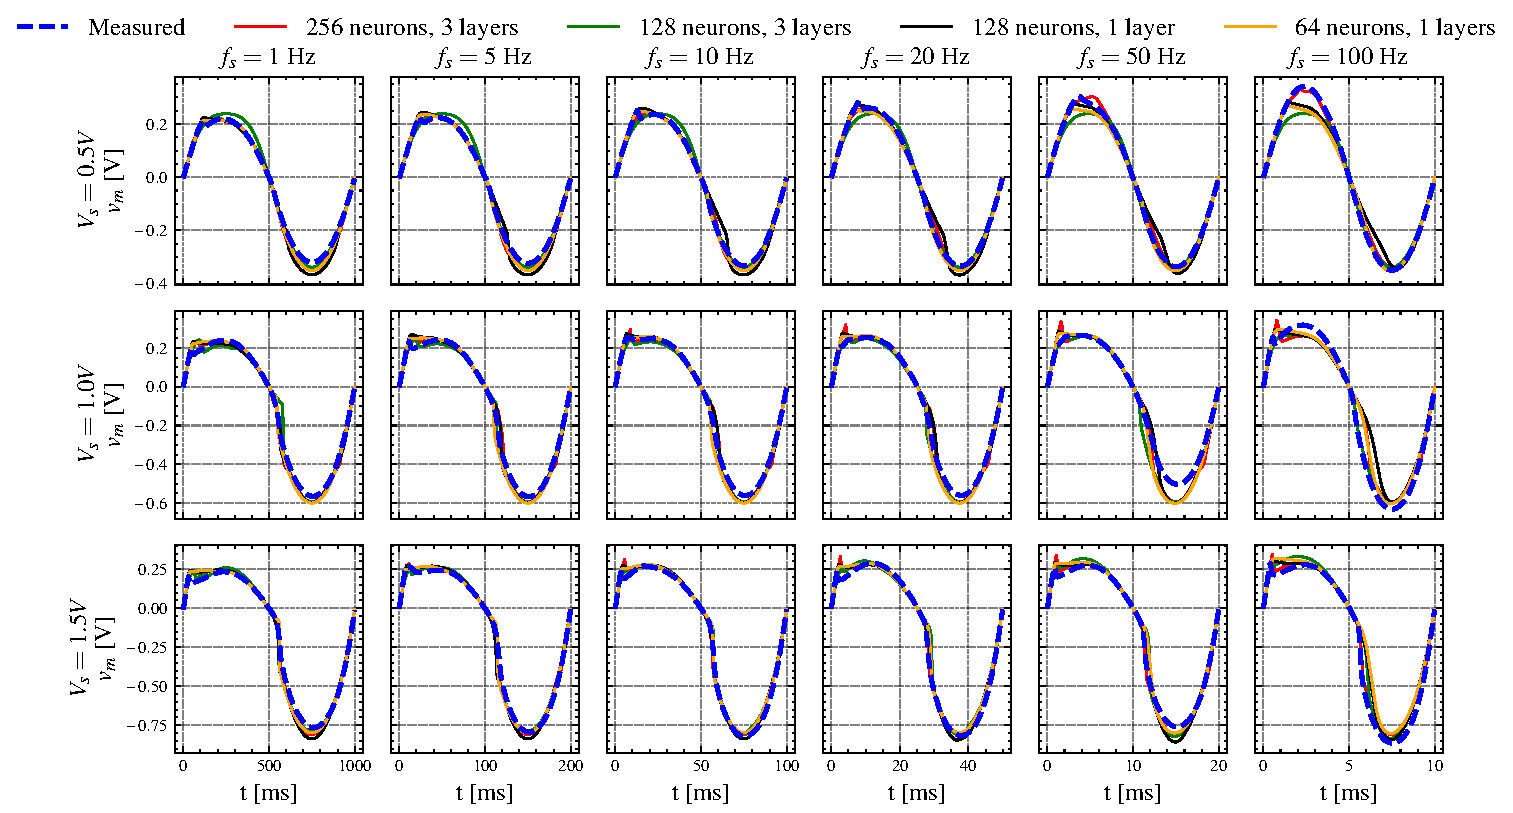
\includegraphics[width=\linewidth]{sample_results/simulated_vms.pdf}
    \caption{Comparative analysis of period-averaged memristor voltage waveforms ($v_m$) across different neural network architectures. The period-averaging process eliminates cycle-to-cycle variations and reveals the fundamental voltage characteristics reproduced by each network configuration. Variations between architectures indicate differences in the models' ability to capture the nonlinear voltage-dependent switching dynamics and internal state evolution of the memristive device.}
\end{figure}

\begin{figure}[htbp!]
    \centering
    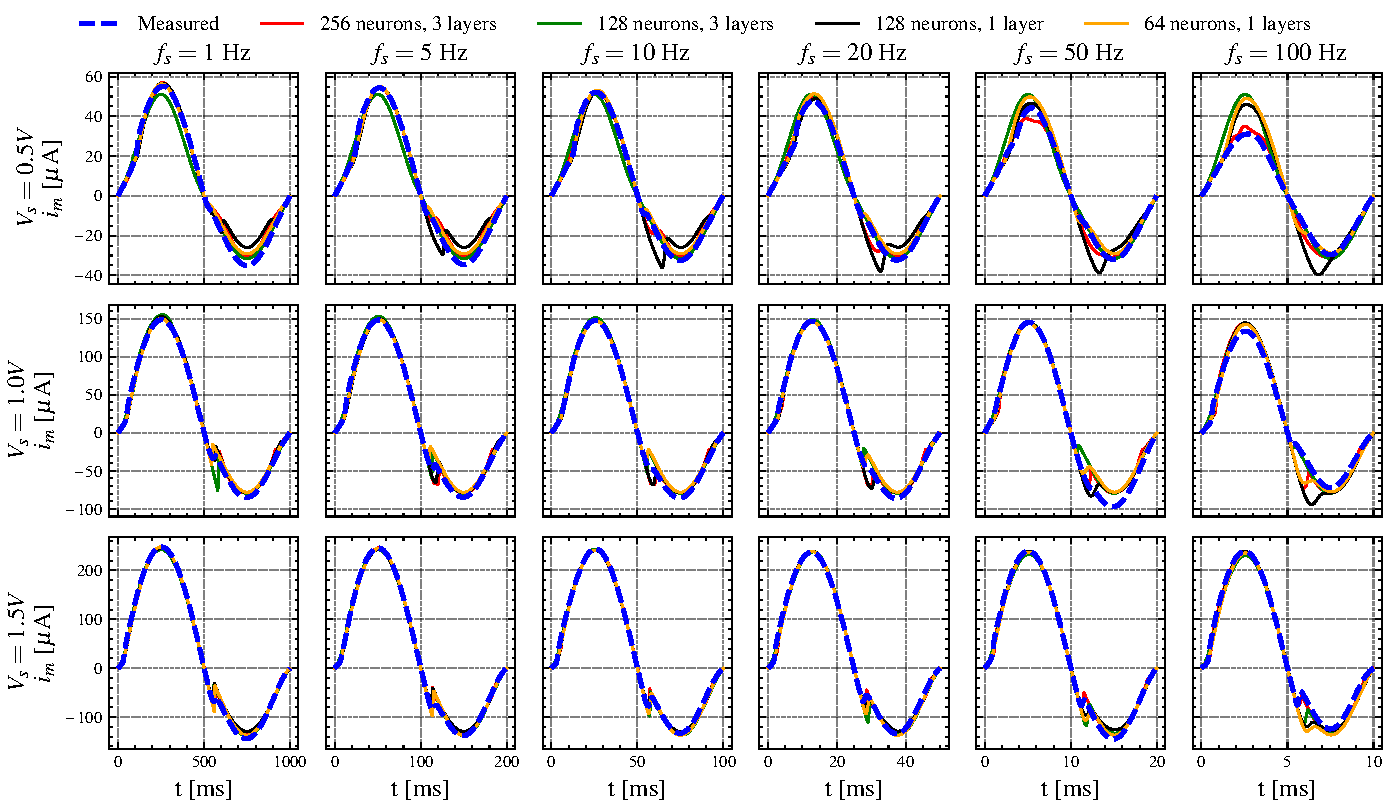
\includegraphics[width=\linewidth]{sample_results/simulated_ims.pdf}
    \caption{Comparative analysis of period-averaged memristor current responses ($i_m$) for various neural network architectures. The current waveforms directly reflect the conductance modulation characteristics and switching kinetics captured by each model. Architectural differences manifest as variations in current amplitude, switching sharpness, and temporal evolution patterns, providing insights into each network's capacity to represent the underlying ionic transport mechanisms governing memristor operation.}
\end{figure}

\begin{figure}[htbp!]
    \centering
    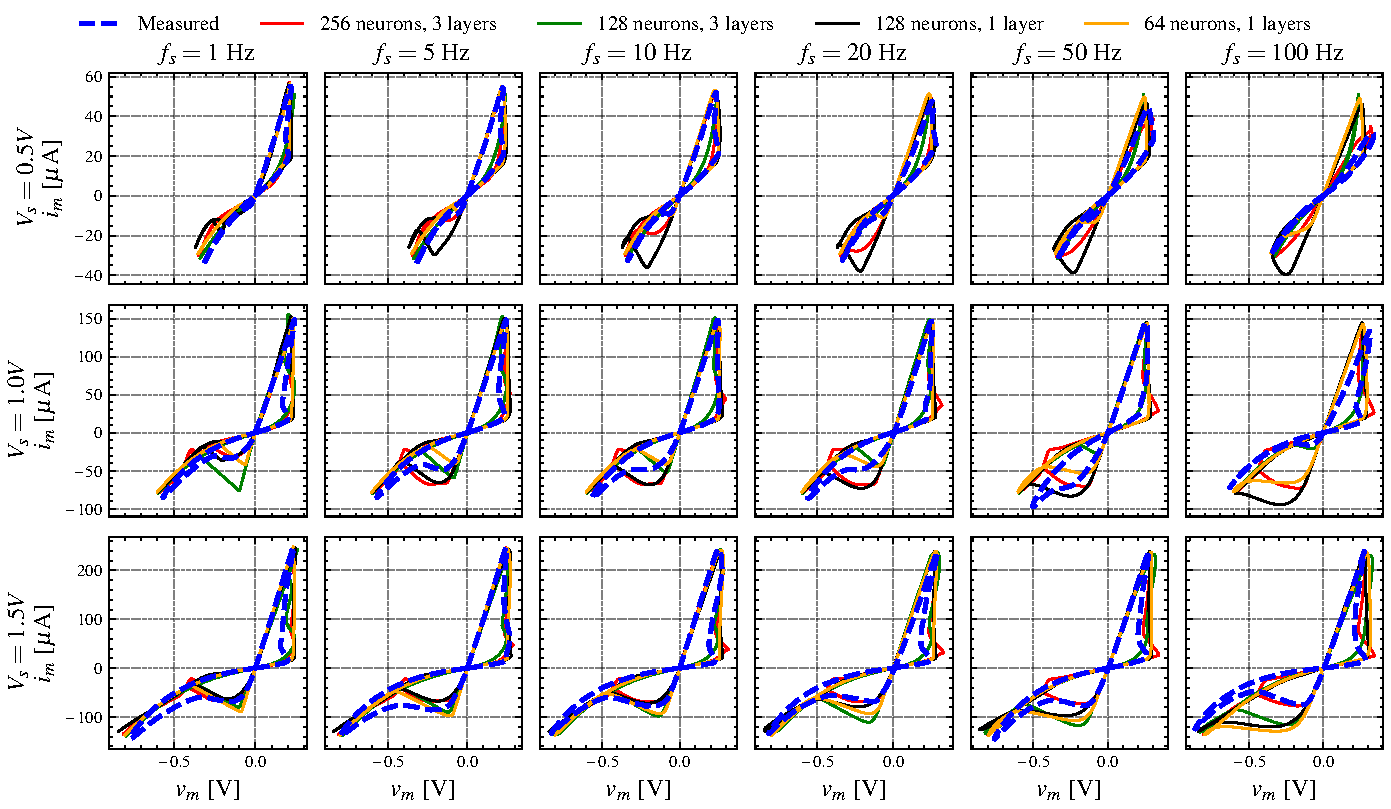
\includegraphics[width=\linewidth]{sample_results/simulated_histeresis.pdf}
    \caption{Comparative analysis of period-averaged voltage-current hysteresis characteristics ($v_m - i_m$) across different neural network architectures. The hysteresis loops represent the most diagnostic feature of memristive behavior, with loop shape, switching thresholds, and pinching characteristics directly reflecting the quality of the neural network's representation of memory-dependent conductance modulation. Architectural variations affect the fidelity of hysteretic reproduction, particularly in the switching transition regions and asymmetric behavior between positive and negative voltage excursions.}
\end{figure}

\begin{figure}
    \begin{subfigure}[c]{0.48\linewidth}
        \centering
        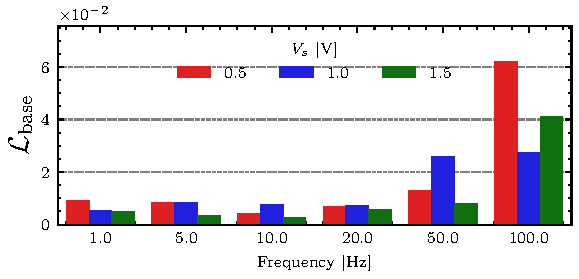
\includegraphics[width=\linewidth]{sample_results/loss_per_freq_model_silu_64_1best_cpu.pdf}
        \caption{64 neurons, 1 hidden layer}
    \end{subfigure}
    \hfill
    \begin{subfigure}[c]{0.48\linewidth}
        \centering
        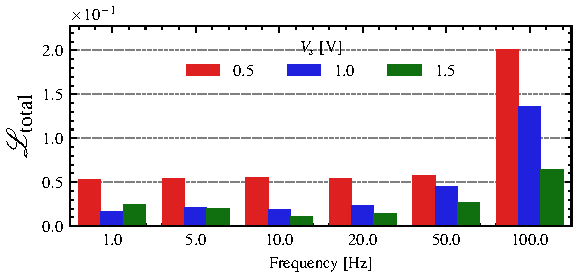
\includegraphics[width=\linewidth]{sample_results/loss_per_freq_model_silu_128_1best_cpu.pdf}
        \caption{128 neurons, 1 hidden layer}
    \end{subfigure}
    \begin{subfigure}[c]{0.48\linewidth}
        \centering
        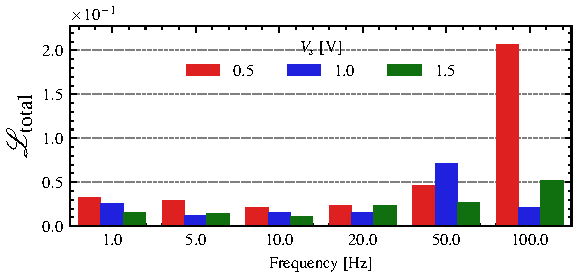
\includegraphics[width=\linewidth]{sample_results/loss_per_freq_model_silu_128_3best_cpu.pdf}
        \caption{128 neurons, 3 hidden layers}
    \end{subfigure}
    \hfill
    \begin{subfigure}[c]{0.48\linewidth}
        \centering
        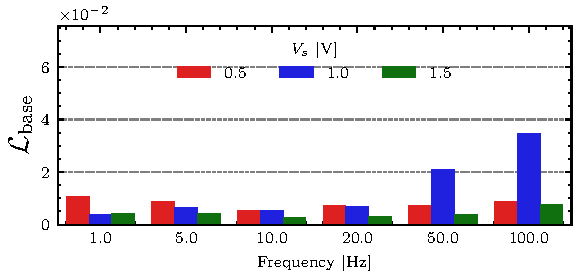
\includegraphics[width=\linewidth]{sample_results/loss_per_freq_model_silu_256_3_cpu.pdf}
        \caption{256 neurons, 3 hidden layers}
    \end{subfigure}
    \caption{Training loss evolution comparison across different neural network architectures demonstrating the relationship between network complexity and learning performance. }
    \label{fig:loss_per_freq}
\end{figure}

The systematic architectural comparison reveals several key insights into the representational requirements for accurate memristor modeling. Network depth influences the ability to capture complex nonlinear transformations associated with ionic transport and structural modifications, while network width affects the dimensionality of the internal representation space available for encoding dynamic state information. The loss function evolution patterns provide quantitative metrics for assessing convergence stability and final model accuracy across the architectural spectrum.

\clearpage

\subsection{Comparative Analysis with Mean Metastable Switch (MMS) Model}

To establish the performance advantages of the neural differential equation approach, a comprehensive comparative analysis was conducted between the developed neural network model and the established Mean Metastable Switch (MMS) memristor model. The MMS model represents a widely accepted analytical framework for memristor behavior that employs metastable state dynamics to describe resistive switching phenomena through probabilistic state transitions and thermal activation mechanisms.

This comparison is particularly significant as the MMS model has been extensively validated against experimental data and serves as a benchmark for memristor circuit simulation in the scientific literature. The comparative evaluation encompasses temporal voltage and current evolution, hysteretic characteristics, and quantitative loss function metrics to provide comprehensive assessment of modeling fidelity across multiple performance dimensions.

Quantitative analysis reveals substantial performance improvements achieved by the neural network approach. The average loss function value for the neural network model was $0.016947$, representing a significant improvement compared to the MMS model's average loss of $0.072356$, and GMMS model $0.035835$. This $4.3x$ reduction in loss indicates markedly superior agreement between neural network predictions and experimental data, demonstrating the enhanced modeling capability achieved through the neural differential equation framework.

The superior performance of the neural network model can be attributed to its capacity for learning complex nonlinear mappings directly from experimental data, whereas the MMS model relies on predetermined phenomenological relationships that may not fully capture the device-specific dynamics and material-dependent switching characteristics inherent in experimental memristor devices.

\begin{figure}[htbp!]
    \centering
    \begin{subfigure}[c]{0.48\linewidth}
        \centering
        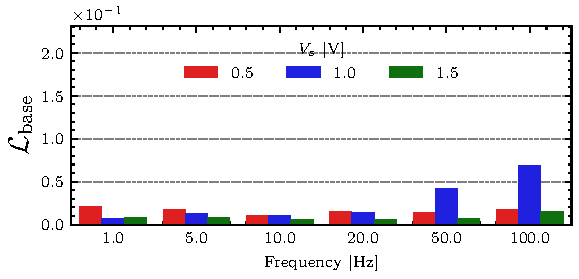
\includegraphics[width=\linewidth]{mms_results/loss_per_freq_256 neurons, 3 layers.pdf}
        \caption{Neural network (256 neurons, 3 hidden layers)}
    \end{subfigure}
    \begin{subfigure}[c]{0.48\linewidth}
        \centering
        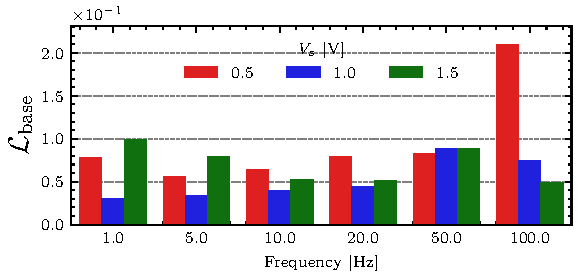
\includegraphics[width=\linewidth]{mms_results/loss_per_freq_MMS Model.pdf}
        \caption{MMS memristor model}
    \end{subfigure}
    \begin{subfigure}[c]{0.48\linewidth}
        \centering
        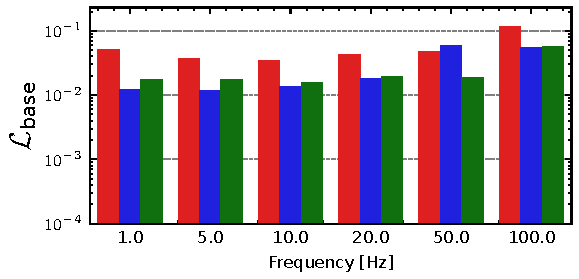
\includegraphics[width=\linewidth]{mms_results/loss_per_freq_GMMS Model.pdf}
        \caption{GMMS memristor model}
    \end{subfigure}
    \caption{Comparative analysis of loss function evolution for (a) the optimal neural network architecture (3 hidden layers, 256 neurons per layer), (b) the Mean Metastable Switch (MMS) model, and (c) the Generalized Mean Metastable Switch (GMMS) model. The neural network demonstrates superior convergence characteristics and achieves significantly lower final loss values, indicating enhanced modeling accuracy and better agreement with experimental memristor dynamics.}
    \label{fig:comparison_mms}
\end{figure}

Representative waveform comparisons between the neural network and MMS models are presented in Figures~\ref{fig:mms_vms}, \ref{fig:mms_ims}, and \ref{fig:mms_histeresis}, providing visual assessment of the modeling differences across key electrical characteristics. These comparisons reveal the neural network's superior ability to capture subtle features of memristor dynamics that are not adequately represented by the phenomenological MMS framework.

\begin{figure}[htbp!]
    \centering
    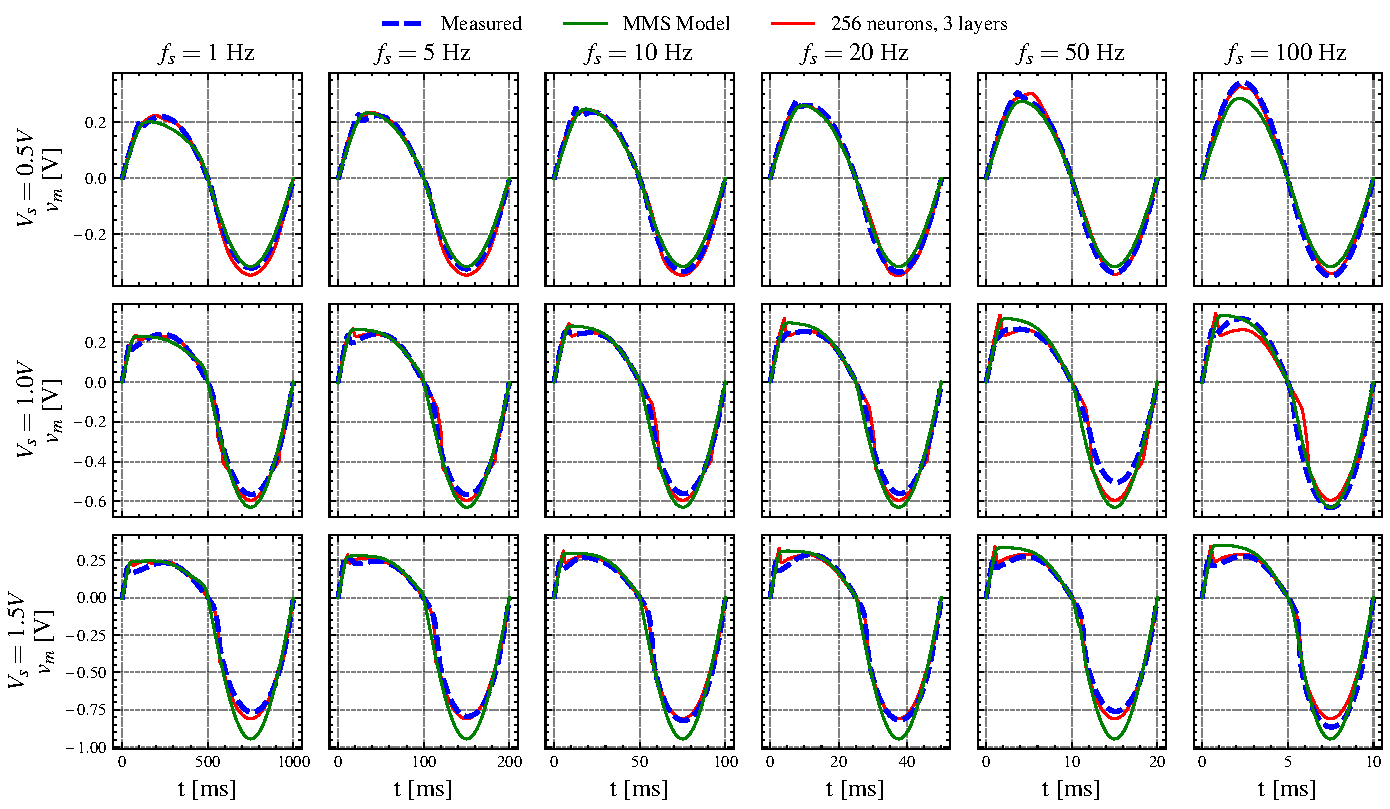
\includegraphics[width=\linewidth]{mms_results/simulated_vms.pdf}
    \caption{Comparative analysis of period-averaged memristor voltage waveforms ($v_m$) between the neural network model and the MMS phenomenological model. The neural network demonstrates superior fidelity in reproducing experimental voltage characteristics, particularly in the transition regions where nonlinear switching dynamics dominate. Differences between the models highlight the enhanced representational capacity of the neural differential equation approach for capturing complex voltage-dependent switching phenomena.}
    \label{fig:mms_vms}
\end{figure}

\begin{figure}[htbp!]
    \centering
    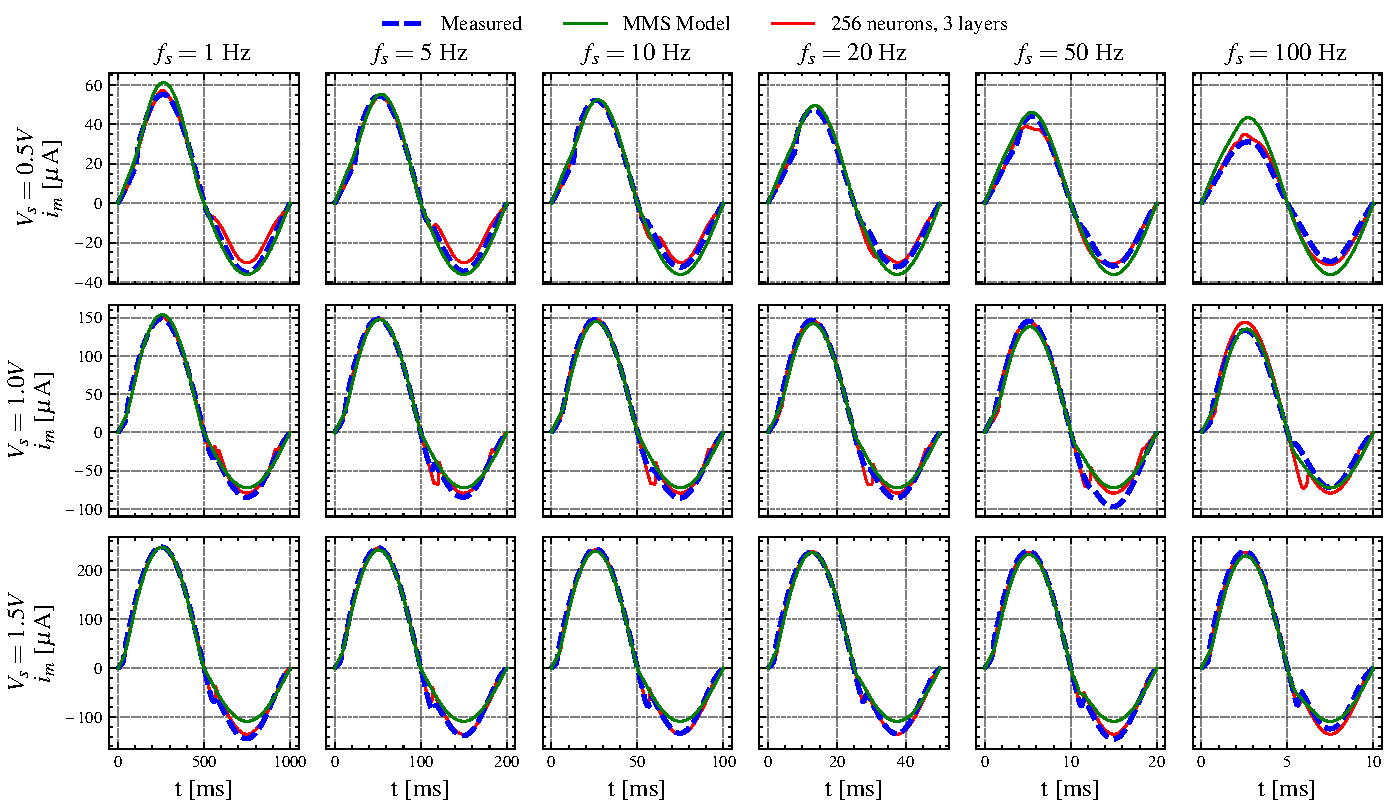
\includegraphics[width=\linewidth]{mms_results/simulated_ims.pdf}
    \caption{Comparative analysis of period-averaged memristor current responses ($i_m$) for the neural network model versus the MMS model. The neural network exhibits superior accuracy in reproducing current switching characteristics, amplitude modulation, and temporal evolution patterns. The enhanced current prediction capability reflects the neural network's ability to learn device-specific conductance modulation mechanisms that extend beyond the assumptions embedded in the MMS phenomenological framework.}
    \label{fig:mms_ims}
\end{figure}

\begin{figure}[htbp!]
    \centering
    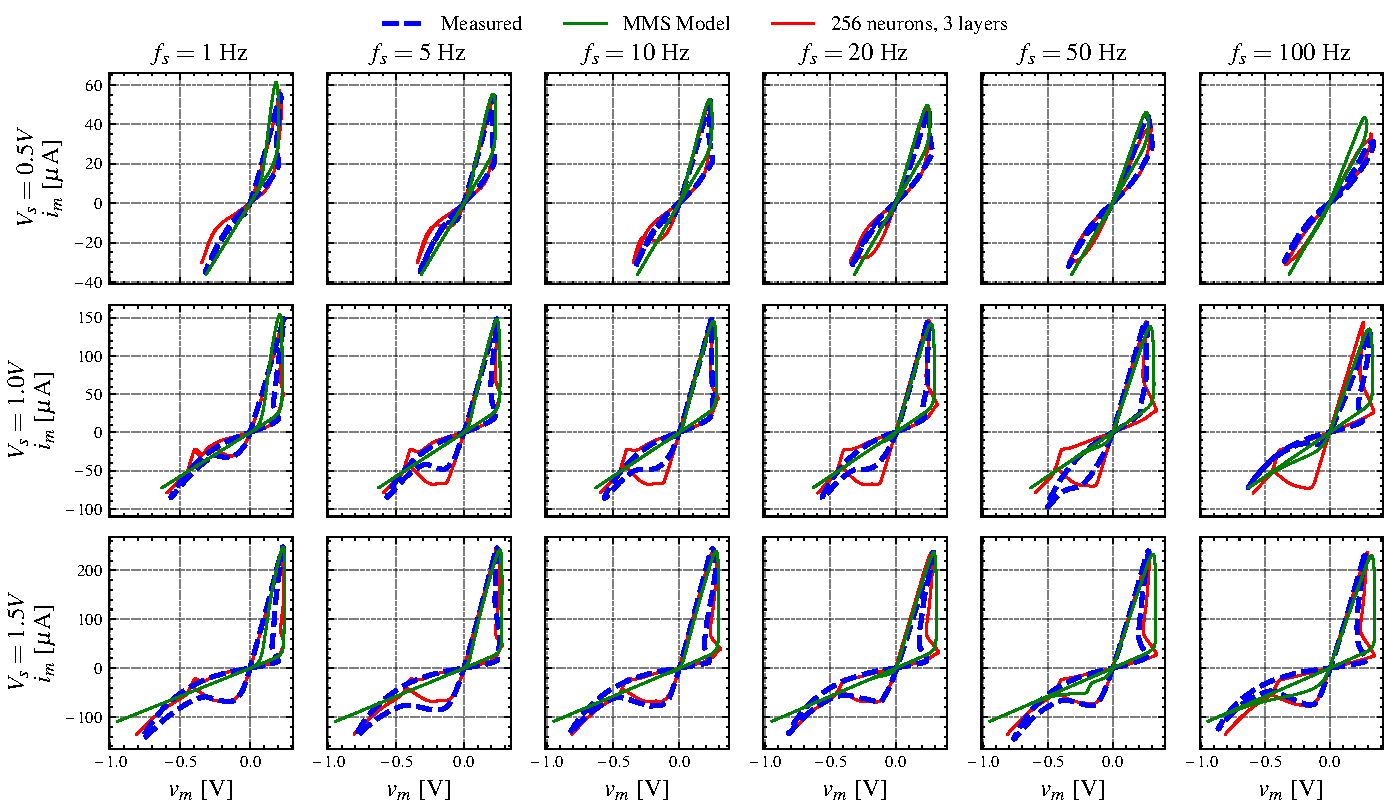
\includegraphics[width=\linewidth]{mms_results/simulated_histeresis.pdf}
    \caption{Comparative analysis of period-averaged voltage-current hysteresis characteristics ($v_m - i_m$) between the neural network and MMS models. The hysteresis loop comparison provides the most diagnostic assessment of modeling quality, as these characteristics directly reflect the memory-dependent conductance properties fundamental to memristive behavior. The neural network demonstrates superior reproduction of loop shape, switching thresholds, and asymmetric behavior, indicating enhanced capture of the underlying physical mechanisms governing resistive switching dynamics.}
    \label{fig:mms_histeresis}
\end{figure}

The comprehensive comparative analysis establishes the neural differential equation approach as a superior methodology for memristor circuit simulation, achieving significant improvements in modeling accuracy while maintaining computational tractability. These results validate the effectiveness of data-driven neural network approaches for capturing complex nonlinear device physics that may be inadequately represented by traditional phenomenological models.

\subsection{Hyperparameter Sensitivity Analysis}

The process of hyperparameter optimization consisted in systematically exploring the space of possible parameter configurations in order to identify those that maximize the predictive performance of the neural network. To this end, the Tree-structured Parzen Estimator (TPE) algorithm was employed, which relies on a probabilistic modeling of the objective function to efficiently balance exploration and exploitation during the search, implemented in the \verb|Optuna| framework~\cite{akiba2019optuna}. The TPE algorithm constructs two separate density models: one for hyperparameter configurations that yield better-than-average performance and another for those that perform worse. By sampling from these models, the algorithm can focus on promising regions of the hyperparameter space while still maintaining diversity in the search process.


Given the sensitivity of neural network performance to hyperparameter selection, a comprehensive hyperparameter optimization procedure was implemented. The search space was designed to cover both architectural and optimization aspects of the model.

Architectural hyperparameters included the number of hidden layers (ranging from $1$ to $5$), layer width ($16$--$512$ neurons, with step size $16$), and activation functions, with candidate functions drawn from common nonlinearities such as ReLU, GELU, SiLU, $\tanh$, ELU, leaky ReLU, sigmoid, as well as identity (linear) and sine functions. The final activation function was restricted to the set $\{\text{linear}, \tanh, \text{sigmoid}, \text{ReLU}\}$.

On the training side, the space included the learning rate for different components (ranging from $10^{-4}$ to $10^{-1}$ on a logarithmic scale), batch size ($1$--$18$), choice of optimizer (Adam, SGD, AdamW, Nadam, AdaBelief), and additional parameters governing regularization and learning rate scheduling (e.g., patience, cooldown, reduction factor, tolerance, and weight decay).

\subsection{MMS Model}

In the MMS model, the optimization were conducted to different set of weights $\lambda_1$, $\lambda_2$, $\lambda_3$, and $\lambda_4$ from ranges $[0, 1]$, $[0, 1]$, $[0, 1]$, and $[0, 1]$, respectively. The parallel plot diagram with pareto front marked has been show in Figure~\ref{fig:mms_hyperparameter_optimization}.


\begin{figure}[H]
    \centering
    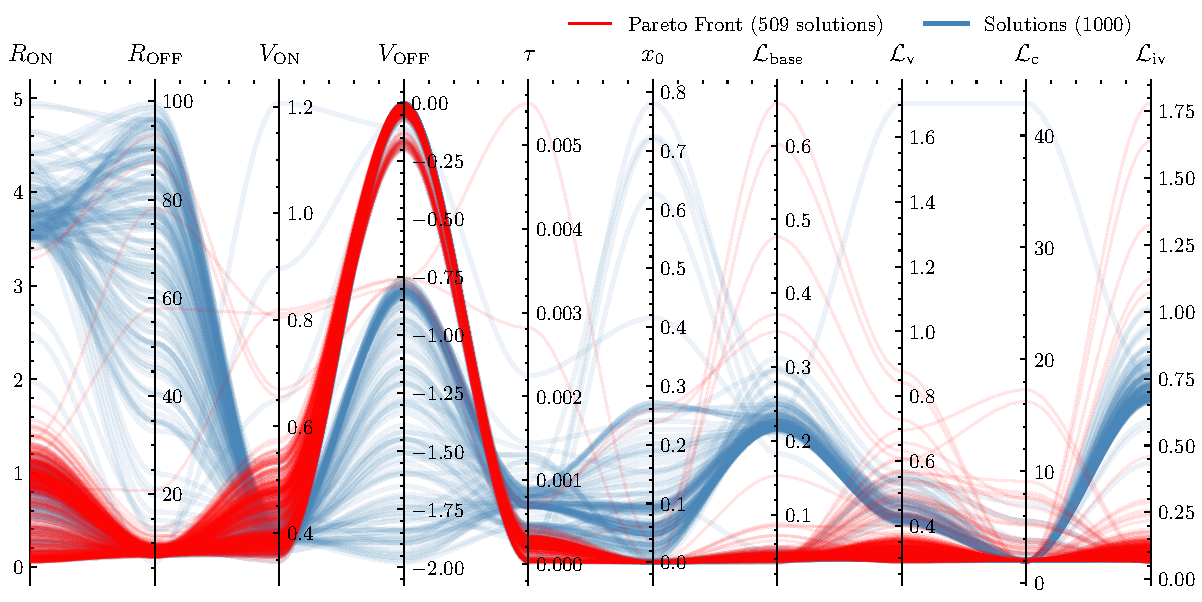
\includegraphics[width=0.8\textwidth]{mms_figs/parallel_coordinates_plot.pdf}
    \caption{Parallel plot diagram with Pareto front for MMS model hyperparameter optimization.}
    \label{fig:mms_hyperparameter_optimization}
\end{figure}


\subsection{Case when memristor resistance is governed by neural network}

When memristor resistance is governed by neural network $\mathcal{M}(\mathbb{x}, v)$, the optimization process must account for the additional complexity introduced by the neural network's architecture and training dynamics. This involves not only tuning the hyperparameters of the neural network itself but also understanding how these parameters influence the memristor's behavior in the context of the overall system. The parallel plot diagram with pareto front marked has been show in Figure~\ref{fig:nn_hyperparameter_optimization}.

\begin{figure}[H]
    \centering
    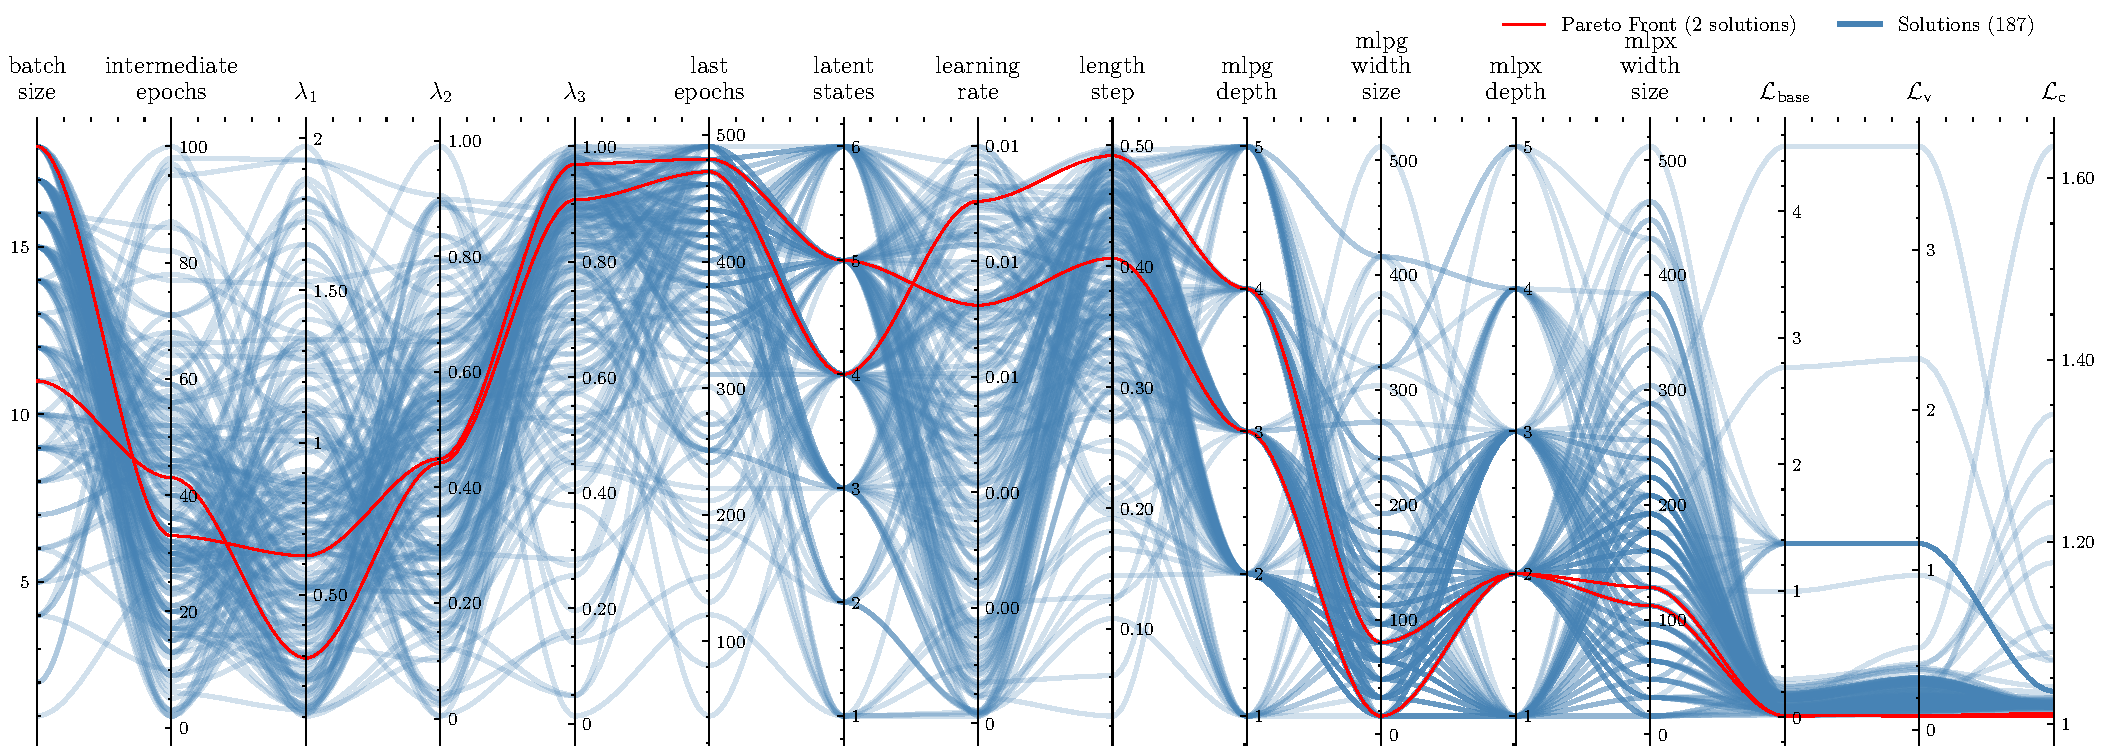
\includegraphics[width=\textwidth]{mms_figs/parallel_coordinates_plot_full.pdf}
    \caption{Parallel plot diagram with Pareto front for neural network model hyperparameter optimization.}
    \label{fig:nn_hyperparameter_optimization}
\end{figure}


\subsection{Case when only memristor state equation is governed by neural network}

When only the memristor state equation is governed by neural network
$\dert{x} = f(x,v_m)$ the optimization process focuses on tuning the hyperparameters that directly affect the state dynamics of the memristor. This includes parameters related to the neural network architecture, such as the number of layers, neurons per layer, and activation functions, as well as training parameters like learning rate, batch size, and optimizer choice. The parallel plot diagram with pareto front marked has been show in Figure~\ref{fig:nn_state_hyperparameter_optimization}.


\begin{figure}[H]
    \centering
    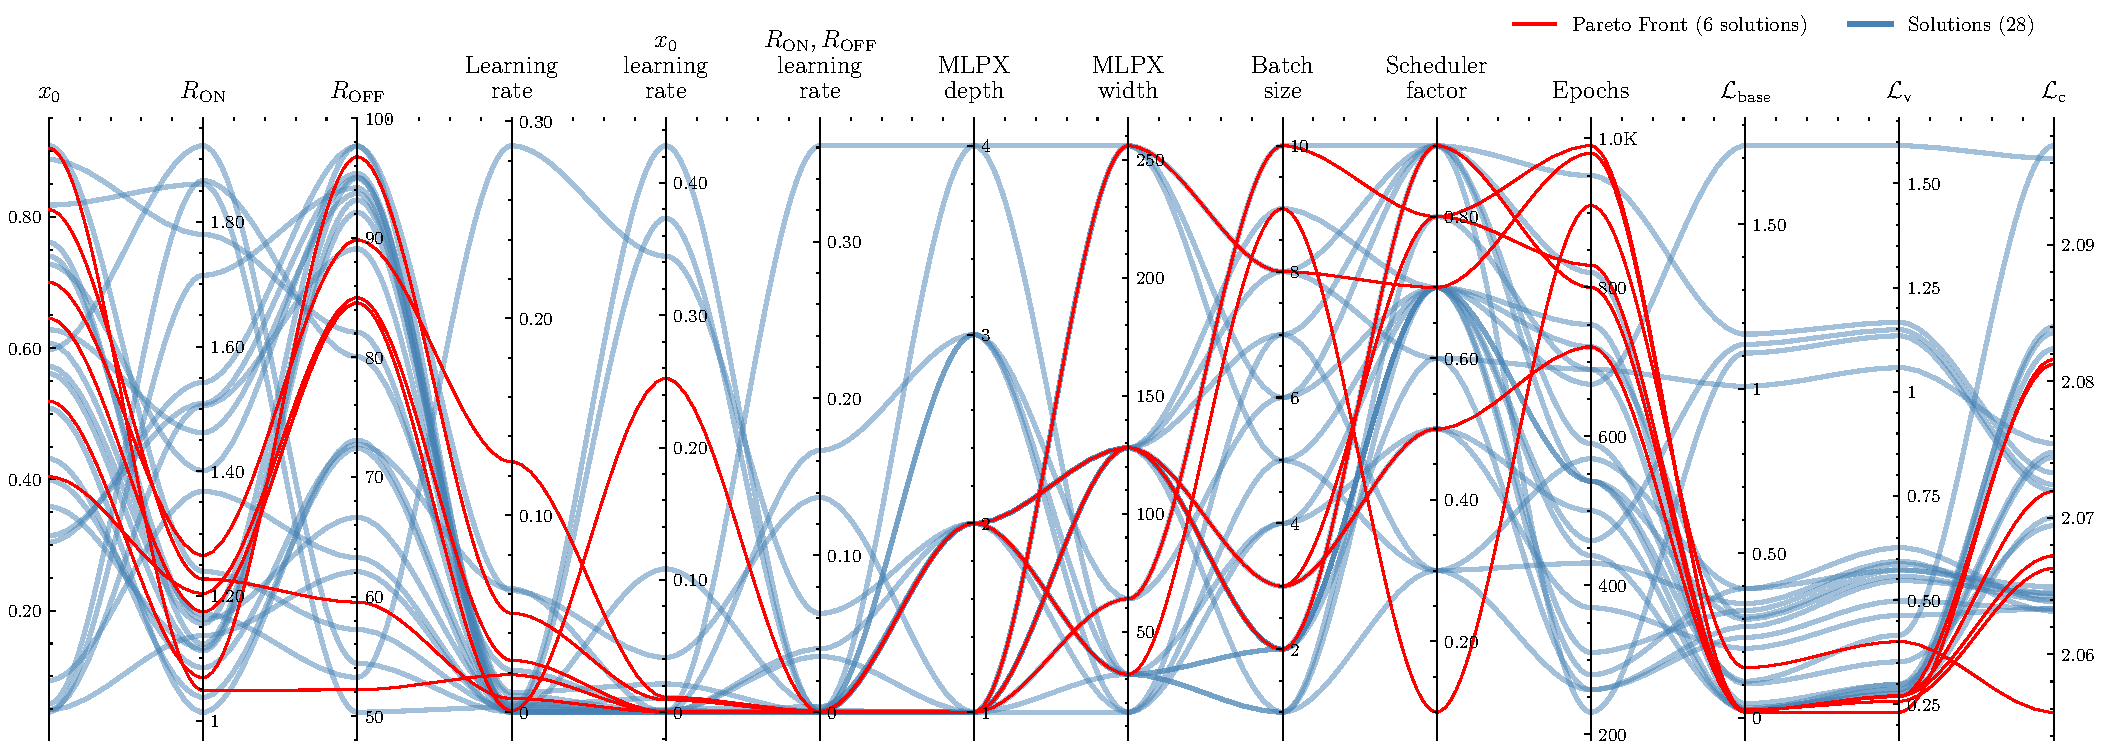
\includegraphics[width=\textwidth]{mms_figs/parallel_coordinates_plot_mlpx.pdf}
    \caption{Hyperparameter optimization parallel plot diagram with Pareto front marked for neural network modeling only dynamic of the internal state variable.}
    \label{fig:nn_state_hyperparameter_optimization}
\end{figure}



\clearpage
\printbibliography[heading=bibintoc]

\end{document}
